\documentclass[a4paper,12pt]{scrreprt}

\usepackage{graphicx}

\usepackage[ngerman]{babel}
\usepackage[T1]{fontenc}
\usepackage{float}
\usepackage[utf8]{inputenc}
\usepackage{subfigure} 
\usepackage{floatflt}
\usepackage{wrapfig}
\usepackage{setspace}
\usepackage{listings}	
\usepackage{courier}
\usepackage{multirow}
\usepackage{xcolor}

\newcommand\digitstyle{\color{lightgreen}}
\makeatletter
\newcommand{\ProcessDigit}[1]
{%
  \ifnum\lst@mode=\lst@Pmode\relax%
   {\digitstyle #1}%
  \else
    #1%
  \fi
}
\makeatother

\colorlet{punct}{red!60!black}
\definecolor{background}{RGB}{255,255,255}
\definecolor{delim}{RGB}{20,105,176}
\definecolor{lightgreen}{HTML}{09885f}
\definecolor{green}{HTML}{008000}
\definecolor{red}{HTML}{a31515}
\colorlet{numb}{magenta!60!black}

\setlength{\parindent}{0em} 
\bibliographystyle{plain}
 
\title{Diplomarbeit: Katzenfütterungsanlage}
\author{Florian Greistorfer, Florian Harrer, Dominik Pichler, Julian Wolf}
\date{Arnfels, \today{}}
\begin{document}
\onehalfspace
\maketitle
\setcounter{tocdepth}{5}
\setcounter{secnumdepth}{4}

\lstdefinestyle{JavaStyle}{
  language=Java,
  columns=flexible,
  frame=single,
  frameround=tttt,
  showstringspaces=false,
  basicstyle=\footnotesize\ttfamily
}

\lstdefinelanguage{json}{
    basicstyle=\footnotesize\ttfamily,
    showstringspaces=false,
    breaklines=true,
    frame=single,
    frameround=tttt,
    backgroundcolor=\color{background},
    literate=
     *{0}{{{\color{numb}0}}}{1}
      {1}{{{\color{numb}1}}}{1}
      {2}{{{\color{numb}2}}}{1}
      {3}{{{\color{numb}3}}}{1}
      {4}{{{\color{numb}4}}}{1}
      {5}{{{\color{numb}5}}}{1}
      {6}{{{\color{numb}6}}}{1}
      {7}{{{\color{numb}7}}}{1}
      {8}{{{\color{numb}8}}}{1}
      {9}{{{\color{numb}9}}}{1}
      {:}{{{\color{punct}{:}}}}{1}
      {,}{{{\color{punct}{,}}}}{1}
      {\{}{{{\color{delim}{\{}}}}{1}
      {\}}{{{\color{delim}{\}}}}}{1}
      {[}{{{\color{delim}{[}}}}{1}
      {]}{{{\color{delim}{]}}}}{1},
}

\lstdefinelanguage{Typescript}{
  keywords={typeof, new, true, false, catch, function, return, null, catch, switch, var, if, in, while, do, else, case, break, class, export, boolean, throw, implements, import, this, constructor, from, =>, public, private, string, new},
  keywordstyle=\color{blue},
  identifierstyle=\color{black},
  sensitive=false,
  comment=[l]{//},
  morecomment=[s]{/*}{*/},
  commentstyle=\color{green}\ttfamily,
  stringstyle=\color{red}\ttfamily,
  morestring=[b]',
  morestring=[b]"
}

\lstdefinestyle{TypescriptStyle}{
   language=Typescript,
   backgroundcolor=\color{white},
   extendedchars=true,
   basicstyle=\footnotesize\ttfamily,
   showstringspaces=false,
   showspaces=false,
   numbers=left,
   numberstyle=\footnotesize,
   numbersep=9pt,
   tabsize=2,
   breaklines=true,
   showtabs=false,
   captionpos=b,
   literate={ä}{{\"a}}1 {ö}{{\"o}}1 {ü}{{\"u}}1
   {0}{{{\ProcessDigit{0}}}}1
   {1}{{{\ProcessDigit{1}}}}1
   {2}{{{\ProcessDigit{2}}}}1
   {3}{{{\ProcessDigit{3}}}}1
   {4}{{{\ProcessDigit{4}}}}1
   {5}{{{\ProcessDigit{5}}}}1
   {6}{{{\ProcessDigit{6}}}}1
   {7}{{{\ProcessDigit{7}}}}1
   {8}{{{\ProcessDigit{8}}}}1
   {9}{{{\ProcessDigit{9}}}}1
   {<=}{{\(\leq\)}}1,
   morestring=[b]",
   morestring=[b]',
   morecomment=[l]//,
}

\tableofcontents
\lohead{Florian Greistorfer}
\chapter{Webserver und Client}

%\begin{figure}[H]
%	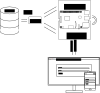
\includegraphics[width=1\textwidth]{Bilder/SVGS/Communication}
%	\caption{Kommunikationen innerhalb des Projekts}
%	\label{kommunikation}
%\end{figure}

\section{Begriffserklärungen}
\label{sec:begriffserklaerung}

\subsection{Server}
\label{sec:begrr-server}
Ein Programm, das Zugriff auf eine Resource oder einen Dienst in einem Netzwerk ermöglicht

\subsection{Client}
\label{sec:begrr-client}
Ein Programm das auf einen Server zugreift

\section{Anforderungen}
\label{sec:anforderungen}

\subsection{Webserver}
\label{sec:anf-server}
Auf der Katzenfütterungsanlage läuft ein Webserver, der es ermöglicht, dass der Benutzer das Gerät über das Internet erreichen kann. Hauptaufgaben des Servers sind dabei, Daten bereitzustellen, zu verabeiten und zu speichern und den Webclient zur Verfügung zu stellen.

\subsection{Client}
\label{sec:anf-client}
Der Client soll dem Benutzer ermöglichen, die Katzenfütterungsanlage über einen Webbrowser zu steuern. Ein Benutzername und ein Passwort sind erforderlich, damit man das Gerät bedienen kann. Das Design soll eindeutig und übersichtlich gehalten sein. Auf der Startseite sollen die eingestellten Fütterungszeiten zu sehen sein und eine allgemeine Übersicht. Über eine Navigationsleiste sollen die weiteren Seiten erreichbar sein:

\begin{itemize}
\item[•]Fütterrungszeiten
\item[•]Positionsinfo
\item[•]Geräteinfo
\item[•]Update
\end{itemize}

\section{Voruntersuchung}
\label{sec:voruntersuchung}

\subsection{HTTP/HTTPS}
\label{sec:vor-http}
Das \ac{HTTP}\footnote{Weitere Informationen zu \ac{HTTP} unter \url{https://developer.mozilla.org/de/docs/Web/HTTP}} ist der Kommunikationsstandart auf dem das Internet basiert. Eine HTTP Session wird über eine Anfrage über das \ac{TCP} an einen Server auf den Port 80 initiiert. Der Server, der auf diesem Port auf eine Anfrage wartet sendet eine Statusmeldung wie z.B. \inlinecode{bash}{HTTP/1.1 200 OK} und eventuell eine eigene Nachricht zurück. Diese Nachricht ist meist die angeforderte Resource oder eine Fehlermeldung. \ac{HTTPS} ist die verschlüsselte Version von \ac{HTTP}. Die meist gebrauchten Anfragen sind:

\begin{itemize}
\item[•] \textbf{GET}: Fordert eine Repräsentation der Ressource an. Ein GET Request darf nur Daten abfragen und darf keinen anderen Einfluss haben.
\item[•] \textbf{PUT}: Fordert das Speichern der Daten, die sich im Request-Body befinden, an. Wenn bereits eine Ressource an der angegebenen \ac{URI} existiert, so wird diese aktualisiert, sonst wird die Resource erstellt.
\item[•] \textbf{POST}: Fordert das Speichern der Daten, die sich im Request-Body befinden, unter der angegebenen \ac{URI} an. 
\item[•] \textbf{DELETE}: Fordert das Löschen der Ressource unter der angegebenen \ac{URI} an.
\end{itemize}

\subsubsection{HTTP Status Codes}
\label{sec:http-status-codes}
\begin{itemize}
\item[•] \textbf{1xx}: Information
\item[•] \textbf{2xx}: Erfolg
\item[•] \textbf{3xx}: Umleitung
\item[•] \textbf{4xx}: Client Fehler
\item[•] \textbf{5xx}: Server Fehler
\end{itemize}

\subsection{JavaScript}
\label{sec:vor-js}
JavaScript ist die Programmiersprache des Internets. Jeder herkömmliche Browser ist in der Lage, JavaScript auszuführen. Mit JavaScript ist es möglich, das Aussehen einer Webseite während der Laufzeit zu ändern, Dinge zu entfernen, hinzufügen und animieren. JavaScript ist heute eine objektorientierte Sprache. Es hebt sich von anderen Sprachen vor allem dadurch ab, dass die Datentypen von Variable nicht fix sind. Das bedeutet, wenn eine Variable den Datentyp \textit{number} hat und es wird ein String angehängt, verändert sich der Datentyp automatisch auf \textit{string}. JavaScript kann nur in einem Thread laufen, das bedeutet, es gibt kein echtes Multithreading. Damit etwas Ähnliches erzielt werden kann, gibt es die Möglichkeit von Callback Methoden. Diese werden ausgeführt, sobald etwas vorher abgeschlossen wurde. Damit ist es möglich, Dinge, die länger brauchen, im ''Hintergrund'' laufen zu lassen\footnote{Mehr information zu Callbacks, Promises und JavaScript unter \url{https://www.w3schools.com/js/default.asp}}.

\subsection{Node.js}
\label{sec:vor-node}
Node.js ist eine Laufzeitumgebung, die es ermöglicht, dass Javascript direkt auf einem Rechner ausgeführt werden kann. Node.js kommt mit dem \ac{npm}. Mithilfe diesem Tools ist es möglich, Module zu installieren, updaten, löschen und veröffentlichen. Diese Module werden im Ordner \textit{/node\_modules} installiert und in der Datei \textit{package.json} unter \textit{dependencies}, oder mit der option \inlinecode{bash}{--save-dev} unter \textit{dev-dependencies} eingetragen. Ein neues Projekt erstellt man mit \inlinecode{bash}{npm init}. Dieses Tool erstellt die Datei \textit{package.json}, in der alle Abhängigkeiten und Informationen über das Projekt stehen. Wenn man ein Projekt kopiert, braucht man den \textit{/node\_modules} Ordner nicht mit kopieren. Man muss nur im Zielordner einmal \inlinecode{bash}{npm install} aufrufen.

\subsection{TypeScript}
\label{sec:vor-ts}
TypeScript ist eine, von Microsoft entwickelte, Weiterentwicklung von JavaScript. Das bedeutet, jeder gültige JavaScript Code ist auch ein gültiger TypeScript Code. TypeScript wird vom TypeScript Compiler in sauberes JavaScript übersetzt. TypeScript ist sehr gut für größere Anwendungen geeignet. Typescript hat strenge Datentypen, Klassen und Vererbung. Die Datentypen von TypeScript sind:

\begin{itemize}
\item[•] \textbf{string}: eine Unicode codierte Zeichenkette, von JavaScript übernommen
\item[•] \textbf{number}: eine vorzeichenbehaftete Gleitkommazahl, kann auch hexadezimal, octal oder binär sein, von JavaScript übernommen
\item[•] \textbf{boolean}: true oder false, von JavaScript übernommen
\item[•] \textbf{array}: eine Liste von Elementen des gleichen Datentyps, von JavaScript übernommen
\item[•] \textbf{tuple}: eine Liste von Elementen unterschiedlichen Datentyps deren Anzahl bekannt ist
\item[•] \textbf{enum}: eine Möglichkeit, numerischen Werten Namen zu geben
\item[•] \textbf{any}: Datentyp unbekannt, wird behandelt wie in JavaScript
\item[•] \textbf{void}: kein Datentyp, meist Rückgabewert bei Funktionen
\item[•] \textbf{null}: leerer Wert, kann allen anderen zugewiesen werden, von JavaScript übernommen
\item[•] \textbf{undefined}: kein Wert, kann allen anderen zugewiesen werden, von JavaScript übernommen
\item[•] \textbf{never}: wenn ein Wert niemals auftreten kann z.B. eine Funktion die immer einen Fehler produziert
\end{itemize}

Damit JavaScript Module von TypeScript verwendet werden können, benötigen sie sogenannte Type Annotations. Diese können bei den meisten bekannteren Modulen über den \ac{npm} installiert werden. Diese Pakete haben den Namenspräfix \textit{@types/}, das bedeutet, dass zum Beispiel die Type Annotations des Express Moduls über \inlinecode{bash}{npm install --save-dev @types/express} installiert werden können. Sollten keine Type Annotations für ein Modul vorhanden sein, muss man diese selbst erstellen.

\subsection{express}
\label{sec:vor-express}
Express ist ein Javascript Modul, dass auf dem Node.js Modul \textit{http} bzw \textit{https} aufbaut. In diesen Modulen ist bereits alles enthalten, dass benötigt wird, um einen Webserver zu programmieren. Express nimmt uns die meiste Arbeit ab und bietet viele weitere Möglichkeiten\footnote{Weitere Information zu express unter \url{https://expressjs.com/}}.

\subsection{JSON}
\label{sec:vor-json}
\ac{JSON} ist die Textrepräsentation eines JavaScript Objekts\footnote{Weitere Informationen zu \ac{JSON} unter \url{https://www.json.org/}}. Die möglichen Datentypen sind:

\begin{itemize}
\item[•] \textbf{string}: 0 oder mehrere unicode Zeichen innerhalb Doppelhochkommas
\item[•] \textbf{boolean}: true oder false
\item[•] \textbf{number}: Eine vorzeichenbehaftete Zahl, die auch die E Notation unterstützt z.B. 0.2E4 (=2000)
\item[•] \textbf{Array}: Eine geordnete Liste von 0 oder mehreren Werten innerhalb eckiger Klammern, Elemente sind getrennt durch Kommas.
\item[•] \textbf{Object}: Eine ungeordnete Sammlung von Name-Wert-Paaren, wo die Namen, die auch Keys genannt werden, Strings sind. Jeder Key sollte eindeutig sein. Innerhalb geschwungener Klammern. Paare sind durch Komma getrennt
\item[•] \textbf{null}: Ein leerer Wert
\end{itemize}

\begin{lstlisting}[style=JSON,caption=\ac{JSON} Beispiel]
{
	"Object": {	
		"string": "name",
		"number": 10E5,
		"boolean": true,
		"Array": [
			{
				"string": "wert",
				"number": 1
			},
			{
				"string": "wert",
				"number": 2
			}
		]
	}
}
\end{lstlisting}

\subsection{JSON Web Token}
\label{sec:vor-jwt}
\ac{JWT} ist ein JSON-basierter, offener Standard für das erstellen von Access Tokens. Mithilfe eines \ac{JWT} kann ein Client sich ausweisen. Ein \ac{JWT} wird vom Server entweder mit einem Secret oder seinem privaten Schlüssel signiert. Dadurch können Server und Client beide überprüfen, ob der Token legitim ist. Ein \ac{JWT} besteht aus drei Teilen. Dem Header, der Payload und der Signature. Im Header steht der fürs Verschlüsseln der Signatur benutzte Algorithmus z.B: \inlinecode{JSON}{\{"alg":"RS256","typ":"JWT"\}}. Im Payload stehen die Daten, die entweder den Client ausweisen oder ähnliche Information. Beispiel: \inlinecode{JSON}{\{"user": "cat", "iat": 1520875121, "exp": 1520911121\}} \textit{iat} bedeutet \textit{issued at} und sagt aus, wann der Token generiert wurde. In der Signature steht der Key, der unsignierte Token, das ist der Header und die Payload Base64 codiert, und die Signatur. Alle drei Teile werden Base64 codiert und mittels Punkt voneinander getrennt.

\subsection{MongoDB}
\label{sec:vor-mongo}
MongoDB ist eine schemenlose Datenbank. Schemenlos bedeutet, dass die Datenbank, im Vergleich zu schemenbehafteten Datenbanken, keine klare Strukturierung benötigt. Einer schemenlosen Datenbank kann man einfach Daten geben und wieder abfragen. Eine schemenbehaftete Datenbank ist in Zeilen und Spalten unterteilt. Diese müssen vorher feststehen. Da Raspian, das Betriebssystem vom Raspberry Pi, nur 32 Bit ist und MongoDB ab Version 3 nur mehr in 64 Bit erhältlich ist, mussten wir auf eine ältere Version wechseln. Die Verbindung der MongoDB Datenbank erfolgt über einen Driver. Der Driver muss mit der Datenbankversion übereinstimmen. MongoDB ist ein \ac{DBMS}, das bedeutet, ein Server läuft auf dem Port 27017, über den alle Datenbanken im System erreichbar sind z.B. die Datenbank \textit{fuettr} ist über \inlinecode{bash}{localhost:27017/fuettr} erreichbar. Eine Gruppe von Daten nennt man Collection. Zugriff auf die Datenbank erfolgt serverseitig wie folgt:

\begin{lstlisting}[caption=Verbinden mit dem \ac{DBMS},style=TS]
const dbServer = await mongodb.MongoClient.connect(url);
\end{lstlisting}

\begin{lstlisting}[caption=Auswählen der Datenbank,style=TS]
const dbFuettr = await dbServer.db('fuettr');
\end{lstlisting}

\begin{lstlisting}[caption=Auswählen der Collection,style=TS]
const collTimes = await dbFuettr.collection('data_times');
\end{lstlisting}

\begin{lstlisting}[caption=Auslesen aller Datensätze mit einem Identifier,style=TS]
const Times = await this._times.find({ identifier: 'Times' }).toArray();
\end{lstlisting}

\begin{lstlisting}[caption=Überschreiben eines Datensatzes mit einem Identifier,style=TS]
this._times.updateOne({ identifier: 'Times' }, { $set: times });
\end{lstlisting}

\subsection{DOM}
\label{sec:vor-dom}
Das \ac{DOM} ist die Objektrepräsentation des \ac{HTML} Dokuments. Durch das \ac{DOM} kann eine JavaScript Anwendung \ac{HTML} Elemente ändern, entfernen, und hinzufügen, \ac{HTML} Attribute ändern, entfernen und hinzufügen und \ac{CSS} Styles ändern. Das \ac{DOM} wird vom Browser beim Laden der Website erstellt. 

\subsection{Angular 2/4}
\label{sec:vor-angular}
Angular ist ein TypeScript Framework, das aus dem Javascript-Framework AngularJS weiterentwickelt wurde. Es wird von Google entwickelt. Angular ist gegliedert in Module. Die grobe Struktur wird in der Abbildung \ref{Angular Struktur} dargestellt\footnote{Genauere Informationen und Tutorials unter \url{https://angular.io/}}.

\begin{figure}[H]
      \includegraphics[width=1\textwidth]{Bilder/Greistorfer/Angular}
      \caption[Angular Struktur]{Angular Struktur\protect\footnotemark}
      \label{Angular Struktur}
\end{figure}

\footnotetext{\autoref{Angular Struktur} Quelle: \url{https://angular.io/guide/architecture\#whats-next} (besucht am 10.3.2018)}

\subsubsection{Modules}
\label{sec:ang-modules}
Jede Angular App ist in \textit{Module}s gegliedert. \textit{Module}s fassen meist ähnliche Funktionen zusammen. Jede App muss mindestens ein \textit{Module} enthalten. Dies heißt standardmäßig \textit{AppModule}. Ein \textit{Module} ist die größte Einheit einer Angular App.  Ein \textit{Module} kann folgende Komponenten beinhalten:

\begin{itemize}
\item[•]Services
\item[•]Andere Module
\item[•]View Classes
\begin{itemize}
\item[-]Components
\item[-]Directives
\item[-]Pipes
\end{itemize}
\end{itemize}

\subsubsection{Libraries}
\label{sec:ang-libraries}
Eine Angular Library ist ein Modul, das \textit{Modules} exportiert. Diese können von \textit{Components} und \textit{Modules} importiert werden. Der Name jeder Angular library beginnt mit \textit{@angular}. Angular libraries können mit dem \ac{npm} installiert werden.

\subsubsection{Components}
\label{sec:ang-components}
Ein \textit{Component} kontrolliert einen Teil des Bildschirms, den sogenannten \textit{view}. Die Logik des \textit{Component}s wird in einer Klasse definiert. Die Klasse interagiert mit dem \textit{view} durch eine \ac{API} von Eigenschaften und Methoden.

\paragraph*{Lifecycle Hooks}\mbox{}\\
Ein Lebenszyklus in Angular ist immer der Lebenszyklus des jeweiligen \textit{Components}. Ein \textit{Component} kann erstellt, verändert und zerstört werden. Zu jedem Stadium gibt es eine Methode, die automatisch je nach Stadium von Angular aufgerufen werden. Die am häufigsten verwendeten sind:

\begin{itemize}
\item[•] \textbf{OnInit()}: Wird aufgerufen, wenn der \textit{Component} erstellt wird. Die dazugehörige Methode ist \inlinecode{TS}{ngOnInit()}. Zeitaufwendige Operationen sollten hier aufgerufen werden, anstatt im constructor, da das den Erzeugungsvorgang verlangsamen würden.
\item[•] \textbf{OnDestroy()}: Wird aufgerufen, wenn der \textit{Component} zerstört wird. Die dazugehörige Methode ist \inlinecode{TS}{ngOnDestroy()}. Hier sollten alle laufenden Prozesse, wie Intervals und Callbacks beendet werden.
\item[•] \textbf{OnChanges()/DoCheck()}: Werden aufgerufen, wenn sich irgentetwas an der \textit{Component} ändert. Die dazugehörige Methoden sind \inlinecode{TS}{ngOnChanges()} und \inlinecode{TS}{ngDoCheck()}.
\end{itemize}

Alle Lifecycle Hooks müssen von der Klasse mit \inlinecode{TS}{implements} implementiert und von \textit{@angular/core} importiert werden.

\subsubsection{Templates}
\label{sec:ang-templates}
Das Aussehen des \textit{view}s wird in einem \textit{Template} definiert. Ein \textit{Template} ist eine \ac{HTML} Datei, mit Angular's Template Syntax. Das bedeutet, dass einige Zusatzbefehle vorkommen können. Beispiele hierfür sind:

\begin{itemize}
\item[•]*ngFor
\item[•]*ngIf
\item[•]\{\{variable\}\}
\item[•](click)
\item[•][variable]
\item[•]<app-route>
\end{itemize}

Die meisten Zusatzbefehle werden für \textit{Data Binding} verwendet.
\newpage
\mbox{}
\begin{wrapfigure}{l}{0.5\textwidth}
\vspace{-50pt}
  \begin{center}
    \includegraphics[width=0.4\textwidth]{Bilder/Greistorfer/databinding}
  \end{center}
  \caption[Angular Databinding]{Angular Databinding\protect\footnotemark}
  \label{Angular Databinding}
  \vspace{0pt}
\end{wrapfigure}
\vspace{-40pt}

\footnotetext{\autoref{Angular Databinding} Quelle: \url{https://angular.io/guide/architecture-components\#data-binding} (besucht am 10.3.2018)}

\subsubsection{Data binding}
\label{sec:ang-data-binding}
Ohne Framework wäre der Programmierer dafür verantwortlich, sicherzustellen, dass Daten in \ac{HTML} Elemente geschrieben werden und dass auf Benutzerinteraktionen reagiert wird. Das ist aufwendig, Fehleranfällig und schwer zu lesen. Angulars Lösung dafür nennt sich \textit{data binding}. Der Programmierer muss nur mehr im \ac{HTML} Template Angular mitteilen, wie die beiden Seiten verbunden werden sollen. In der Abbilung \ref{Angular Databinding} sind die vier möglichen Arten von \textit{data binding} dargestellt. Jede Art hat eine Richtung, vom \ac{DOM} zum \ac{DOM} oder in beide Richtungen.

\begin{itemize}
\item[•] \inlinecode{Html}{<span>\{\{variable\}\}</span>} Der Wert der Variable in den Klammern wird anstelle des Klammerausdrucks dargestellt. Wenn sich der Wert ändert, ändert sich auch der Wert im \ac{DOM}
\item[•] \inlinecode{Html}{<span [hidden]="hide"></span>} übergibt den Wert in der angegebenen Variable in das angegebene Attribut
\item[•] \inlinecode{Html}{<span (click)="clicked(\$event)"></span>} ruft die angegebene Methode auf, wenn das angegebene Event auftritt.
\item[•] \inlinecode{Html}{<input [(ngModel)]="variable">} der Wert im Eingabefeld und in der Variable sind voneinander abhängig, ändert sich der eine, so ändert sich der andere zum gleichen
\end{itemize}

\subsubsection{Services}
\label{sec:ang-services}
Services sind Klassen, die eine Aufgabe erfüllen, unabhängig von allem anderen. Sie werden vor allem verwendet, wenn eine Aufgabe etwas Zeit erfordert, wie z.B. eine Serveranfrage. Services bieten auch die Möglichkeit, dass \textit{Components} Zugriff auf eine gemensame Variable haben, da Angular keine globalen Variablen hat. Services müssen vom \textit{Dependency Injector} injiziert werden. Der \textit{Dependency Injector} indiziert alle Abhängigkeiten in eine \textit{Component}.

\subsection{Angular CLI}
\label{sec:vor-angular-cli}
Das Angular \ac{CLI} ist ein JavaScript Modul, das über den \ac{npm} installiert werden kann. Mithilfe des \ac{CLI} ist das erstellen und übersetzen von Angular Anwendungen um vieles erleichtert. Ein neues Projekt erstellt man mit \inlinecode{bash}{ng new <projektname>} und übersetzt wird mit \inlinecode{bash}{ng build}. Mit der Option \inlinecode{bash}{--prod} wird die Anwendung kompakter und für den Einsatz im produktiven Umfeld übersetzt.

\subsection{Bootstrap}
\label{sec:vor-bootstrap}
Bootstrap ist eine CSS Bibliothek, die die Möglichkeit bietet, bereits vorgefertigte Komponenten auf unserer Website zu verwenden. An erster Stelle stehen bei Bootstrap responsive Design und Mobilgeräte. Responsive bedeutet, dass die Elemente sich an die breite des Bildschirms anpassen. Dadurch erspart man sich als nicht sehr designaffiner Programmierer viel Arbeit. Auf der offiziellen Bootstrap Website kann man außerdem verschiedene Themes auswählen. Bootstrap wurde von Twitter entwickelt und ist entweder über den \ac{npm} oder über Bootstraps eigenes \ac{CDN} erhältlich.

\section{Umsetzung}
\label{sec:umsetzung}

\subsection{Projektstruktur}
\label{sec:ums-projektstruktur}
\dirtree{%
.1 Webserver.
.2 server.
.3 dist.
.3 keys.
.3 node\_modules.
.3 public.
.3 src.
.4 views.
.2 ngx.
.3 dist.
.3 e2e.
.3 node\_modules.
.3 src.
.4 app.
.5 components.
.5 services.
.4 assets.
.4 environments.
.4 i18n.
}

Das Projekt ist so strukturiert, dass eine klare Trennung zwischen Client und Server herrscht.
\paragraph*{Server} Im \textit{keys} Ordner befinden sich der öffentliche und private Schlüssel, die vom install Script erstellt werden. Im \textit{public} Ordner befinden sich die Ressourcen, die direkt vom Server gesendet werden, z.B. Fehlermeldungsseiten. Im \textit{src} Ordner sind die TypeScript Arbeitsdateien. Diese werden in den \textit{dist} Ordner übersetzt.
\paragraph*{Client} Der Client Ordner hat den Namen \textit{ngx}, dass sagt aus, es ist ein Angular Projekt, die Angular Version ist aber egal. Im \textit{src} Ordner befinden sich alle Dateien, die das Angular \ac{CLI} benötigt, um die Anwendung zu bauen. Im \textit{assets} Ordner befinden sich alle Ressourcen, die die Anwendung benötigt, wie z.B. Bilder. Im Ordner \textit{i18n} befinden sich die Dateien, die das \ac{CLI} braucht, um die Anwendung in mehrere Sprachen zu übersetzen. Im \textit{app} Ordner befindet sich die eigentlich Anwendung. Die Anwendung ist klar getrennt in den Ordner \textit{components} und \textit{services}.

\subsection{Client}
\label{sec:ums-client}

\subsubsection{Design}
\label{sec:ums-client-design}
Das Design sollte übersichtlich und einfach gestaltet werden. Der Benutzer soll auf den ersten Blick die wichtigsten Funktionen und Informationen erkennen können. \\

\begin{wrapfigure}{r}{0.7\textwidth}
\vspace{-10pt}
  \begin{center}
    \includegraphics[width=0.65\textwidth]{Bilder/Greistorfer/Home}
  \end{center}
  \caption{Startseite}
  \label{Startseite}
  \vspace{-10pt}
\end{wrapfigure}

Auf der Startseite sind alle wichtigen Informationen übersichtlich dargestellt. Auf der linken Seite werden die Uhrzeit der letzten erfolgreichen Fütterung, die Zeit der nächsten Fütterung und die Zeit bis zur nächsten Fütterung dargestellt. Darunter werden Fehler und Warnungen, falls welche auftreten sollten, angezeigt. Da unbekannt ist, wie viele Fehler und Warnungen auftreten, werden diese in einem *ngFor aufgelistet. Auf der rechten Seite sind die aktiven Fütterungszeiten aufgelistet. \\

\begin{wrapfigure}{r}{0.7\textwidth}
\vspace{-10pt}
  \begin{center}
    \includegraphics[width=0.65\textwidth]{Bilder/Greistorfer/Fuetterungszeiten}
  \end{center}
  \caption{Fütterungszeiten}
  \label{Fütterungszeiten}
  \vspace{-10pt}
\end{wrapfigure}

Auf der Fütterungszeiten-Seite kann der Benutzer die Katzenfütterungsanlage ein und ausschalten. Dies wurde mit einer Checkbox realisiert, die durch Styles wie ein Schalter gestaltet wurde. Darunter können die Fütterungszeiten geändert und deaktiviert werden. Siehe Abbildung \ref{Fütterungszeiten}. Der Button 'Speichern' wird deaktiviert, sobald eine Zeit ungültig eingegeben wurde, oder wenn die Zeiten nicht in aufsteigender Reihenfolge sortiert sind. \newpage

\begin{wrapfigure}{r}{0.7\textwidth}
\vspace{-10pt}
  \begin{center}
    \includegraphics[width=0.65\textwidth]{Bilder/Greistorfer/Gerateinformation}
  \end{center}
  \caption{Geräteinformationen}
  \label{Geräteinformationen}
  \vspace{-60pt}
\end{wrapfigure}

Auf der Geräteinformations-Seite werden die wichtigsten Daten über das Gerät angezeigt. diese Daten sind:
\begin{itemize}
\item[•]Seriennummer
\item[•]Interner Rechner
\item[•]WLAN Status
\item[•]IP Adresse
\item[•]Softwareversion
\end{itemize}
Die IP-Adresse ist die aktuelle \textbf{externe} IP-Adresse. \\

\begin{wrapfigure}{r}{0.7\textwidth}
\vspace{-10pt}
  \begin{center}
    \includegraphics[width=0.65\textwidth]{Bilder/Greistorfer/Update}
  \end{center}
  \caption{Update}
  \label{Update}
  \vspace{-10pt}
\end{wrapfigure}

Auf der Update-Seite kann der Benutzer nach Updates suchen, Updates starten oder die Maschine herunterfahren. Wenn der Benutzer auf den Herunterfahren-Button klickt, der sich auf der linken Seite ganz unten befindet, wird er gewarnt, dass die Maschine nur mehr über das Aus- und wieder Einstecken des Netzteils Startbar ist.\\

\subsubsection{Funktion}
\label{sec:ums-client-funktion}

\paragraph*{Struktur} \mbox {}\\
Der Haupt-\textit{Component}, der geladen wird, wenn die Seite aufgerufen wird, ist \textit{app.component}. In seinem Template ist die Navigationsleiste, die sich alle Seiten teilen. Alle weiteren Seiten werden im \inlinecode{html}{<router-outlet></router-outlet>} angezeigt. Das ist ein \ac{HTML}-Tag der von Angulars Router zur Verfügung gestellt wird. Ein Router ist ein Service, dass das Navigieren der Seite ermöglicht. Damit das funktioniert, muss dem Router mitgeteilt werden, wie die Seite aufgebaut ist. Dies geschieht im \textit{router.module}:

\begin{lstlisting}[caption=Routes Definition,style=TS]
const routes: Routes = [
  { path: 'home', component: HomeComponent, 
  		data: { title: 'Füttr' }, canActivate: [AuthGuard]},
  { path: '', pathMatch: 'full', redirectTo: 'login'},
  { path: 'login', component: LoginComponent,
  		data: { title: 'Füttr - Login' }},
  { path: 'position', component: PositionComponent, 
  		data: { title: 'Füttr - Positions' }, canActivate: [AuthGuard]},
  { path: 'feed', component: FeedComponent, 
  		data: { title: 'Füttr - Feeding-Cycle' }, canActivate: [AuthGuard},
  { path: 'info', component: InfoComponent, 
  		data: { title: 'Füttr - Info' }, canActivate: [AuthGuard]},
  { path: 'update', component: UpdateComponent, 
  		data: { title: 'Füttr - Update' }, canActivate: [AuthGuard]},
  { path: '**', component: Error404Component, 
  		data: { title: 'Füttr - 404 (not found)'}}
];
\end{lstlisting}

Jede Route bekommt ein data Objekt übergeben, dass bei Aufruf der \textit{Component} dem @Input Decorator injiziert wird. Der jeweilige \textit{Component} ändert damit den Titel der Seite. Alle Routes, bis auf \textit{login} und \textit{404} sind von einem AuthGuard geschützt, dass bedeutet, nur authorisierte Benutzer können diese Routes aufrufen. Der Request auf \textit{root} \inlinecode{TS}{path: ''} wird umgeleitet auf \textit{login}. Für jeden Request, dessen Route nicht definiert ist, wird der 404 Component geladen: \inlinecode{TS}{path: '**'}.

\paragraph*{\ac{HTTP} Service}\mbox{}\\
Da alle \textit{Components} Daten vom Server holen und manche auch Daten zum Server schicken, war es die logische Schlussfolgerung, ein Service zu erstellen, das egal welche Art von \ac{HTTP} Anfrage verarbeiten kann. Dieses Service ist \textit{http.service}. Alle Anfragen, egal ob \textit{GET} oder \textit{PUT} werden von diesem Service getätigt. Das Service importiert Angular's \textit{HttpClient}, mit dem es sehr einfach ist, Anfragen zu erstellen und die Antworten zu verarbeiten. Die Antworten vom Server sind vom Typ \textit{application/json}, das bedeutet, sie sind \ac{JSON}-Dateien, die der \textit{HttpClient} dann in Objekte umwandelt. Diese Objekte werden dem \textit{Component} übergeben, sobald die Anfrage abgeschlossen wurde.

\paragraph*{Fütterungszeiten}\mbox{}\\
Die Eingabe wurde realisiert durch \ac{HTML} input Elemente vom Typ \textit{time}. Da \textit{time} Browserabhängig ist und ältere Browser es als \textit{text} interpretieren könnten, und die Application auf allen Browsern funktionieren soll, werden alle Eingabefelder auf Richtigkeit überprüft. Außerdem sollen alle Zeiten in aufsteigender Reihenfolge eingegeben werden. Der \textit{time} Typ ist eigentlich nur ein string, das bedeutet, um die Reihenfolge zu überprüfen, müssen diese zuerst in Zahlen umgewandelt werden. Das geht mit der Funktion \inlinecode{TS}{parseInt()}. Ein string von einem \textit{time} input sieht meistens so aus: \inlinecode{TS}{'12:34'} Wenn die Zeit leer ist, sieht er so aus: \inlinecode{TS}{'--:--'} Auf diese beiden Arten muss unser Parser vorbereitet sein. Der Parser wandelt den string in Minuten um, danach werden sie verglichen. Sollte eine Zeit ungültig sein oder sollte eine Zeit ausser Reihenfolge sein, so wird der Speicher-Button deaktiviert. Überprüft wird, sobald der User etwas ändert. Dies geschieht durch den DoCheck() Lifecycle Hook (siehe \ref{sec:ang-components}). Über den Fütterungszeiten kann man außerdem die Maschine ein und ausschalten. Dies ist realisiert durch eine Checkbox, die mit \ac{CSS} wie ein Schalter gestyled wurde.

\begin{lstlisting}[caption=Zeiten Parser,style=TS,label=zeiten_parser,captionpos=t]
toMinutes(time: string): number {
  let timeHours: number;
  let timeMinutes: number;
  if (time[0] === '-' && time[1] === '-' 
      && time[3] === '-' && time[4] === '-') {
    return null;
  }
  timeHours = parseInt(time[0], 10) * 10;
  timeHours = timeHours + parseInt(time[1], 10);
  timeMinutes = parseInt(time[3], 10) * 10;
  timeMinutes = timeMinutes + parseInt(time[4], 10);
  return timeHours * 60 + timeMinutes;
}
\end{lstlisting}

\paragraph*{Updates}\mbox{}\\
Auf der Updates Seite kann der Benutzer nach neuen Updates suchen und das Gerät updaten. Realisiert wurde dies durch eine Anfrage an Github, wo eine Datei namens \textit{version.json} liegt. Diese wird verglichen mit der Datei, die auf dem System liegt. Dieser Vergleich geschieht bereits im OnInit() Lifecycle Hook (siehe \ref{sec:ang-components}). Der User kann nochmal nach Updates suchen, wenn er dies möchte. Sollte ein Update verfügbar sein, so wird der Button aktiv und der Benutzer kann sich dazu entscheiden, dass Gerät upzudaten. Wird aktualisiert, so wird eine Anfrage an den Server gesendet siehe \ref{sec:ums-server-funktion}. Der Client beginnt, dauerhaft Anfragen zu senden, bis eine fehlschlägt. Eine Nachricht teilt dem Benutzer mit, dass das System aktualisiert. Dann werden so lange Anfragen gesendet, bis wieder eine Antwort ankommt. Dann wird die Seite automatisch neu geladen. Der Updatevorgang ist damit abgeschlossen.

\paragraph*{Login}\mbox{}\\
Das Login funktioniert auf der Basis des Angular Auth Guards. Dieser schützt gewisse Routes gegen unbefugte Benutzer. Im Login bekommen wir, bei erfolgreicher Authentifikation einen \ac{JWT} vom Server, den wir in einer Variable speichern und dann im \inlinecode{bash}{Authorization} Header bei Bedarf mitschicken. Dies geschieht durch einen sogenannten \textit{Interceptor}, der den \ac{HTTP} Request nimmt und ihn klont, da \ac{HTTP} Requests in Angular nicht veränderbar sind, und dann darauf den \inlinecode{bash}{Authorization} Header gibt.

\subsubsection{Internationalization}
\label{sec:ums-client-i18n}
Um die Webseite in mehreren Sprache anzeigen zu können, muss sie in allen Sprachen extra übersetzt sein. Das würde bedeuten, für jede Sprache wird ein eigenes Angular Projekt benötigt. Das wäre sehr viel Speicherplatz und Rechenleistung. Glücklicherweise bietet Angular eine Möglichkeit, die App in mehrere Sprachen zu übersetzen, ohne die ganze App neu zu schreiben. Diese Möglichkeit nennt sich Internationalization oder kurz i18n. Angluar muss nur wissen, welche Teile wie übersetzt werden sollen. Dafür schreiben wir bei allen \ac{HTML} Elementen, deren Text wir übersetzen wollen i18n zu den Attributen. \inlinecode{Html}{<h4 i18n>Zeit 1:</h4>}. Mit dem Kommando \inlinecode{bash}{ng xi18n --output-path src/i18n} werden alle Texte in eine Datei namens messages.xlf extrahiert. Diese Datei kann dan kopiert werden und einem Übersetzer gegeben. Im Falle dieser Arbeit wurden die Texte alle in Deutsch und Englisch übersetzt. Zum bauen des mehrsprachigen Projekts muss Angular mitgeteilt werden, welche Sprachen und welche Dateien es verwenden soll. Unter Linux geht das mit dem Kommando \inlinecode{bash}{for lang in en de; do ng build --output-path}\\\inlinecode{bash}{=dist/\$lang --aot --prod --bh \$lang/ --i18n-file=src/i18n/messages.\$lang.xlf}\\\inlinecode{bash}{--i18n-format=xlf --locale=\$lang; done}

\subsubsection{Kommunikation mit dem Server}
\label{sec:ums-client-kommunikation}
Der Client benötigt viele Daten vom Server und sendet einige an den Server. Das Übertragungsprotokoll, Tabelle \ref{webserver-client-uebertragung}, gibt klare Auskunft über alle mögliche Anfragen und Antworten.
\begin{landscape}
\begin{table}[]
\begin{tabular}{@{}llll@{}}
\toprule
\multicolumn{1}{|l|}{\textbf{\ac{HTTP} Request Typ}} & \multicolumn{1}{l|}{\textbf{\ac{URI}}} & \multicolumn{1}{l|}{\textbf{Server Response}} & \multicolumn{1}{l|}{\textbf{Beispiel}}                                                                                                          \\ \midrule
\multicolumn{1}{|l|}{GET}  & \multicolumn{1}{l|}{/api/ip}                             & \multicolumn{1}{l|}{IP}                  & \multicolumn{1}{l|}{\{''ip":"62.116.40.166"\}}                                                                                                                                                                                                                       \\ \midrule
\multicolumn{1}{|l|}{GET}  & \multicolumn{1}{l|}{/api/version}                        & \multicolumn{1}{l|}{Version}             & \multicolumn{1}{l|}{\{"version": "beta@1.0.0"\}}                                                                                                                                                                                                                     \\ \midrule
\multicolumn{1}{|l|}{GET}  & \multicolumn{1}{l|}{/api/getUpdate}                      & \multicolumn{1}{l|}{200 OK}              & \multicolumn{1}{l|}{}                                                                                                                                                                                                                                                \\ \midrule
\multicolumn{1}{|l|}{GET}  & \multicolumn{1}{l|}{/api/shutdown}                       & \multicolumn{1}{l|}{200 OK}              & \multicolumn{1}{l|}{}                                                                                                                                                                                                                                                \\ \midrule
\multicolumn{1}{|l|}{GET}  & \multicolumn{1}{l|}{/api/callMeMaybe?q=times}            & \multicolumn{1}{l|}{Zeiten}              & \multicolumn{1}{l|}{\begin{tabular}[c]{@{}l@{}}\{"time1":"12:20","time1\_active":true,"time2":"13:20",\\ "time2\_active":true,"time3":"14:20","time3\_active":true,\\ "time4":"15:20","time4\_active":true\}\end{tabular}}                                           \\ \midrule
\multicolumn{1}{|l|}{GET}  & \multicolumn{1}{l|}{/api/callMeMaybe?q=status}           & \multicolumn{1}{l|}{Status}              & \multicolumn{1}{l|}{\begin{tabular}[c]{@{}l@{}}\{"nextFeeding":"-","lastFeeding":''ausstehend",\\"nextFeedingIn":''-'',"machineState":false\}\end{tabular}}                                                                                                            \\ \midrule
\multicolumn{1}{|l|}{GET}  & \multicolumn{1}{l|}{/api/callMeMaybe?q=info}             & \multicolumn{1}{l|}{Info}                & \multicolumn{1}{l|}{\begin{tabular}[c]{@{}l@{}}\{''serialnumber":"17",''internal":"Raspberry Pi 3 Model B",\\ "wlanState":"not connected"\}\end{tabular}}                                                                                                            \\ \midrule
\multicolumn{1}{|l|}{GET}  & \multicolumn{1}{l|}{/api/callMeMaybe?q=positions}        & \multicolumn{1}{l|}{Positionen}          & \multicolumn{1}{l|}{\{"motor1":''-'',"motor2":''-'',''sensor1":''-'',''sensor2":''-''\}}                                                                                                                                                                                         \\ \midrule
\multicolumn{1}{|l|}{GET}  & \multicolumn{1}{l|}{/api/callMeMaybe?q=errors\_warnings} & \multicolumn{1}{l|}{Errors und Warnings} & \multicolumn{1}{l|}{\begin{tabular}[c]{@{}l@{}}\{''Errors":{[}\{"message":''Error","hidden":false\},\\ \{"message":''Error2","hidden":false\}{]},\\ "Warnings":{[}\{"message":"Warning","hidden":false\},\\ "message":"Warning2","hidden":false\}{]}\}\end{tabular}} \\ \midrule
\multicolumn{1}{|l|}{POST} & \multicolumn{1}{l|}{/api/putMeHere?q=times}              & \multicolumn{1}{l|}{Zeiten}              & \multicolumn{1}{l|}{\begin{tabular}[c]{@{}l@{}}\{"time1":"12:20","time1\_active":true,"time2":"13:20",\\ "time2\_active":true,"time3":"14:20","time3\_active":true,\\ "time4":"15:20","time4\_active":true\}\end{tabular}}                                           \\ \midrule
\multicolumn{1}{|l|}{POST} & \multicolumn{1}{l|}{/api/putMeHere?q=changeState}        & \multicolumn{1}{l|}{Status}              & \multicolumn{1}{l|}{\{''state":"true"\}}                                                                                                                                                                                                                             \\ \midrule
\multicolumn{1}{|l|}{POST} & \multicolumn{1}{l|}{/login}                              & \multicolumn{1}{l|}{\ac{JWT}}          & \multicolumn{1}{l|}{\{"token":"...",''isLoggedIn":true\}}                                                                                                                                                                                                             \\ \midrule
\multicolumn{1}{|l|}{POST} & \multicolumn{1}{l|}{/logout}                             & \multicolumn{1}{l|}{200 OK}              & \multicolumn{1}{l|}{}                                                                                                                                                                                                                                                \\ \bottomrule
\end{tabular}
\caption{Übertragungsprotokoll Webserver - Webclient}
\label{webserver-client-uebertragung}
\end{table}
\end{landscape}

\subsection{Server}
\label{sec:ums-server}

\subsubsection{Serverpfade}
\label{sec:ums-server-pfade}

\paragraph*{GET}\mbox{}\\
\begin{forest}
	[\textit{root}
		[api
			[version]
			[callMeMaybe
				[?q{=}times]
				[?q{=}status]
				[?q{=}info]
				[?q{=}positions]
				[?q{=}errors\_warnings]			
			]
			[getUpdate]
			[shutdown]
			[ip]		
		]
		[de]
		[en]
	]
\end{forest}

\paragraph*{POST}\mbox{}\\
\begin{forest}
	[\textit{root}
		[api
			[putMeHere
				[?q{=}times]
				[?q{=}changeState]			
			]	
		]
		[login]
		[logout]	
	]
\end{forest}


\subsubsection{Funktion}
\label{sec:ums-server-funktion}
Da auf einem Port nur ein Programm auf Anfragen warten kann und sichergestellt sein soll, dass der Server nur einmal gestartet wird, wird der Server als Singleton ausgeführt. Das bedeutet, der Konstruktor der Klasse ist nicht öffentlich. Stattdessen gibt es einen Getter, der überprüft, ob ein Objekt der Klasse bereits existiert. Sollte ein Objekt bereits erstell sein, so wird dieses zurückgegeben. Existiert noch kein Objekt, so wird eines erstellt und danach zurückgegeben. Der Server wir gestartet, indem dem Node.js Modul \textit{http} das Server Objekt übergeben wird: \inlinecode{TS}{const server = http.createServer(this._express).listen(port)}

\begin{lstlisting}[caption=Server Singleton,label=server_singleton,style=TS]
public static get Instance(): Server {
  if (Server._instance === undefined) {
    Server._instance = new Server();
  }
  return Server._instance;
}
\end{lstlisting}

Der Server wurde mit dem JavaScript Modul \textit{express} programmiert. Express ist aufgebaut mit sogenannten Middlewares. Diese werden bei eintreffen einer Anfrage der Reihe nach durchgegangen, bis eine Middleware der Anfrage entspricht. Wenn z.B. die Anfrage \inlinecode{bash}{HTTP/1.1 GET /api/version} eintrifft, werden die Middlewares nach der Reihe durchgegangen. Jede Middleware mit \inlinecode{TS}{use}, solange kein Pfad mit angegeben wurde, wird ausgeführt, alle anderen werden übersprungen. Die nächste Middleware, die ausgeführt wird, ist \inlinecode{TS}{get('/api/version', ...)}. Wird in dieser Middleware \inlinecode{TS}{next()} aufgerufen, so werden alle weiteren Middlewares durchgegangen. Sollte \inlinecode{TS}{next()} nicht aufgerufen werden, so werden keine weiteren Middlewares durchgegangen.

\begin{lstlisting}[style=TS,caption=Middlewares,label=middlewares]
this._express.use(bodyparser.json());
this._express.use(bodyparser.urlencoded({ extended: true }));
this._express.use(
  requestLanguage({
    languages: ['en-GB', 'de-DE', 'de-AT']
  })
);
this._express.set('views', path.join(__dirname, '/views'));
const pugEngine = this._express.set('view engine', 'pug');
pugEngine.locals.pretty = true;
this._express.use(this.logger);
this._express.use(express.static(path.join(__dirname, '../public')));
this._express.use('/assets', express.static(path.join(__dirname, '../../ngx/dist/assets')));
this._express.post('/login', (req, res, next) => this.login(req, res, next));
this._express.post('/logout', (req, res, next) => this.logout(req, res, next));
this._express.use('/api', ApiRoutes.ApiRouter.Routes);
this._express.use('/', AppRoutes.AppRouter.Routes);
\end{lstlisting}

Die beiden Middlewares \inlinecode{TS}{bodyparser.json()} und \inlinecode{TS}{bodypareser.urlencoded()} bereiten den Request so auf, dass er vom Rest der Middlewares verstanden werden kann. Die Middleware \inlinecode{TS}{requestLanguage()} ist ein JavaScript Modul, dass aus dem Request-Header den Header \inlinecode{bash}{Accept-Language} ausliest und für die weitere Verarbeitung in \inlinecode{TS}{req.language} speichert. Pug Engine ist eine rendering Engine, das bedeutet, damit können \ac{HTML} Seiten während der Serverlaufzeit generiert werden, somit können Variablen eingefügt werden. \inlinecode{TS}{express.static()} stellt ein Verzeichnis mit allen Unterverzeichnissen zur Verfügung. Das gleiche Prinzip wie bei einem Apache Webserver. Die beiden Seiten des Servers, die Client Seite, und die \ac{API} sind in eigene Dateien ausgelagert. Somit herrscht ein klare Trennung zwischen dem, was der Benutzer zu sehen bekommt und dem, das nur die JavaScript Applikation sieht. Alle \textit{get} und \textit{post} Middlewares haben eine Callback Methode. In dieses bearbeiten wir alle Anfragen und beantworten sie.

\begin{lstlisting}[caption=Sprachenauswahl,style=TS,label=sprachenauswahl]
public languageselector(req: express.Request, res: express.Response, next: express.NextFunction) {
  if (req.language === 'de-DE' || req.language === 'de-AT') {
    res.redirect('/de');
    return;
  } else {
    res.redirect('/en');
    return;
  }
}
\end{lstlisting}

Wenn eine Anfrage auf \textit{root} (/) eintrifft, entscheidet der Server, ausgehend von dem Wert, der in \inlinecode{TS}{req.language} steht, in welcher Sprache der Benutzer die Webseite zu sehen bekommt. Ist der Wert entweder \textit{de-De} oder \textit{de-AT}, so wird die deutsche Seite angezeigt, bei allen anderen Werten, wird die englische Seite angezeigt. Dies geschieht durch weiterleiten des Requests auf entweder \textit{/de} oder \textit{/en}. 

\begin{lstlisting}[style=TS,caption=Login Methode,label=login]
public async login(req: express.Request, res: express.Response, next: express.NextFunction) {
  let User: Login = { token: '', isLoggedIn: false };
  let done = false;
  const username = req.body.user;
  const userpass = SHA512(req.body.password).toString();
  const Users = await FuettrDB.Instance.getUsers();
  for (let i = 0; i < Users.length; i++) {
    let name = JSON.parse(JSON.stringify(Users[i])).user_name;
    let pass = JSON.parse(JSON.stringify(Users[i])).user_password;
    if (userpass === pass && username === name) {
      jwt.sign({ user: username }, this._privkey, { expiresIn: '10h', algorithm: 'RS256' }, (err, token) => {
        if (err != undefined) {
          log.warn(err);
        }
        if (token != undefined) {
          User.token = token;
          User.isLoggedIn = true;
          res.send(JSON.stringify(User));
          done = true;
        }
      });
    }
  }
  setTimeout(() => {
    if (!done) {
      res.status(401).send(JSON.stringify(User));
    }
  }, 2000);
}
\end{lstlisting}

In der Login Methode wird zuerst das im Request befindliche Passwort gehashed. Dann werden alle Benutzer aus der Datenbank ausgelesen und mit dem Benutzer im Request verglichen. Sind Benutzername und Passworthash gleich, so wird mit der Methode \inlinecode{TS}{jwt.sign()} ein \ac{JWT} erstellt und signiert. Dieser Token wird in ein Objekt gepackt und dem Client als Antwort gesendet. Wird innerhalb einer Zeitspanne von zwei Sekunden keine Übereinstimmung gefunden, so sendet der Server den Status 401 (Unauthorized). 




\subsubsection{MongoDB}
\label{sec:ums-server-mongo}
Alle Daten, die nicht direkt vom Java-Programm benötigt werden, werden in eine Datenbank gespeichert. Über diese Datenbank haben sowohl das Java-Programm als auch der Webserver Zugriff auf die gemeinsamen Daten wie die Fütterungszeiten und Geräteinformationen. Da MongoDB eine Schemenlose Datenbank ist, können wir die Daten einfach dem \ac{DBMS} übergeben und sie werden gespeichert. Da Zugriff auf die Datenbank ebenfalls nur einmal erfolgen sollte, wurde die Klasse ebenfalls als Singleton ausgeführt. 

\begin{lstlisting}[caption=Verbindung mit der Datenbank,style=TS,label=database-connection]
const url = 'mongodb://localhost:27017/fuettr';
try {
  const dbServer = await mongodb.MongoClient.connect(url);
  const dbFuettr = await dbServer.db('fuettr');
  const collTimes = await dbFuettr.collection('data_times');
  const collUsers = await dbFuettr.collection('data_user');
  const collInfo = await dbFuettr.collection('data_info');
  const collHardware = await dbFuettr.collection('data_hardware');
  .
  .
  .
  this._times = collTimes;
  this._info = collInfo;
  this._hardware = collHardware;
  this._users = collUsers;
  log.info('Database connected.');
} catch (err) {
  throw err;
}
\end{lstlisting}

Die Verbindung mit dem \ac{DBMS} geschieht über die Methode \inlinecode{TS}{MongoClient.connect()}. Da wir uns dazu entschieden haben, jeden Datensatz in eine eigene Collection zu speichern, müssen Anfangs alle Collections den verschiedenen Variablen zugewiesen werden. Beim Verbinden wird außerdem überprüft, ob die Collections leer sind. Ist dies der Fall, so werden Standardwerte in die Collections geschrieben. \\\\

Beim Request auf \textit{/api/getUpdates} soll die Software aktualisiert und das Raspberry neu gestartet werden. Dafür wurde Node.Js' \textit{child\_process} Modul verwendet. Dieses Modul gibt uns die Möglichkeit, Konsolenbefehle innerhalb unserer Serverseitigen JavaScript Anwendung auszuführen. Zuerst wird das Repository aktualisiert mit \inlinecode{bash}{git pull}. Danach wird das System neugestartet mit \inlinecode{bash}{sudo reboot}. Vorher wird in eine Datei, die vom Raspberry Startup Script rc.local überprüft wird, true geschrieben. Wenn in dieser Date true steht, werden beim starten des Raspberry alle Komponenten der Software neu gebaut.


\subsubsection{Kommunikation mit dem Java Programm}
\label{sec:ums-server-java}
Da der Server und das Java-Programm miteinander kommunizieren müssen, war es notwendig, ein Kommunikationsprotokoll zu erstellen. Alle Daten werden im \ac{JSON} Format ausgetauscht. Das Protokoll sieht wie folgt aus:
\begin{table}[H]
\begin{tabular}{|l|l|l|}
\hline
\ac{HTTP} Request Typ   & \ac{URI}            & Server Response                                                                                \\ \hline
PUT                     & /ChangeMachineState & neuer Maschinenstatus                                                                          \\ \hline
GET                     & /errors\_warnings   & \begin{tabular}[c]{@{}l@{}}JSON Objekt mit einem Error und einem \\ Warning Array\end{tabular} \\ \hline
\end{tabular}
\caption{Übertragungsprotokoll Webserver - Java}
\label{uebertragungsprotokoll}
\end{table}

Die Kommunikation mit dem Java-Programm erfolgt über Node.js' eigenes \textit{http} Modul. Das Modul hat Methoden, mit denen Server und Clients erstellt werden können. Die Kommunikation erfolgt über den lokalen Port 666. Auf diesem Port wartet der Server vom Java-Programm auf Anfragen. Der Webserver, der in diesem Falle zum Client wird, sendet einfache \ac{HTTP} \textit{GET} und \textit{POST} Anfragen an den Java-Server. Dieser antwortet dann mit der gewünschten Resource.

\section{Zusammenfassung und Verbesserungsmöglichkeiten}
\label{sec:zusammenfassung}

\subsubsection{Verbesserungsmöglichkeiten}
\label{sec:verbesserung}
Da die Sprache TypeScript erst im Rahmen dieser Diplomarbeit erlernt wurde, sind viele Unreinheiten im Code zu finden. Es wurde sehr viel experimentiert und ausprobiert. Viele Dinge können verbessert werden. Eine umfangreichere Verwendung der Datenbank wäre besser gewesen. In der Datenbank selbst, wäre es besser gewesen, die Benutzer in eine eigene Collection zu tun und alle anderen Daten in einer Collection zusammenzufassen. Außerdem wären andere Namen besser für die Collections gewesen. Ich war dabei allerdings an meinen Kollegen gebunden, der voreilig die Namen und Unterteilungen festlegte, ohne Rücksprache zu halten und im Nachhinein es nicht mehr ändern wollte. Im Client Design kann die Seite für Mobilgeräte optimiert werden.
\chapter{Java-Programm}
\label{sec:java-programm}

\section{Anforderungen}
\subsection{Programm}
Die Hauptaufgabe des Programms ist es dem Benutzer eine Möglichkeit zum Steuern der Katzenfütterungsanlage zu Verfügung zu stellen. Weiters soll das Programm die Motoren steuern und die Sensoren in der Anlage auswerten können. Für diese Aufgabe sollen die IO-Pins am Raspberry verwendet werden.
\subsection{Design - Benutzerinterface}
Das Design der GUI-Fenster soll einfach und übersichtlich gestaltet werden. Auf der Hauptseite, also der Seite die immer zu sehen ist, sollen Informationen dargestellt werden, die dem Benutzer einen schnellen Überblick über den Zustand der Anlage geben. Alle anderen nicht direkt ersichtlichen Funktionen sollen über sinnvoll benamte Menüpunkte erreichbar sein.
Der Benutzer soll mit Hilfe eines kleinen Touchdisplays die Möglichkeit haben die Anlage zu steuern. Deswegen muss darauf geachtet werden, dass alle GUI-Fenster sinnvoll per Touch-Gesten verwenbar sind.
\subsection{Externe Steuerung}
Da die Katzenfütterungsanlage die Katze füttern soll, wenn die Familie der Katze auf Urlaub ist, sollte die Anlage auch über das Internet erreichbar sein. Dafür gibt es die Möglichkeit einen Benutzer auf der Anlage anzulegen mit welchem man anschließend über eine Webseite auf die Anlage zugreifen kann. Weiters soll das Java Programm (Server) mit der Web-Applikation (Client) kommunizieren, also Daten austauschen, können.

\newpage

\section{Voruntersuchung}
\subsection{Wieso Java und nicht C?}
Zu Beginn musste entschieden werden mit welcher Programmiersprache gearbeitet werden soll. Zur Auswahl standen Java und C.
Vorteile von C:
\begin{itemize}
\item[1] Echtzeitfähige Steuerung der Motoren und Senosren
\item[2] Hardwarenahe Programmierung für die Pins
\end{itemize}
Vorteile von Java:
\begin{itemize}
\item[1] Erstellen einer GUI ist einfacher
\item[2] Implementieren eines Servers ist einfacher
\end{itemize}

Nach dem Gegenüberstellen der Vorteile wurde Java als Programmiersprache gewählt.

\subsection{Wieso das Raspberry Pi 3 Model B?}
Schon zu Beginn der Diplomarbeit war klar, dass mit deinem Raspberry gearbeitet werden soll. Nun musste entschieden werden welches Model verwendet werden soll. Wir haben das Raspberry Pi 3 Model B aufgrund folgender technischer Daten gewählt:
\begin{itemize}
\item[1] Rechenleistung
\item[2] Anzahl der GPIO-Pins
\item[3] WLAN-Fähigkeit
\end{itemize}

\subsection{Auswahl eines Touchdisplays}
Das Display muss folgendet Anforderungen erfüllen:
\begin{itemize}
\item[1] Es muss ein Touchscreen-Display sein
\item[2] Es muss einfach an das Raspberry anschließbar sein
\item[3] Es sollte nicht zu teuer sein
\end{itemize}

Aufgrund dieser Anforderungen wurde das Touchdisplay von Raspberry gewählt.

\subsection{Wieso pi4j?}
Da Java als Programmiersprache gewählt wurde, musste eine Möglichkeit die GPIO-Pins anzusteuern gefunden werden.
Da bei der Recherche außer pi4j Java kaum etwas gefunden wurde, wurde pi4j gewählt. Weiters vorteilhaft ist, dass das Ansteuern der Pins via Code nicht sehr kopliziert ist. 

\subsection{Wieso Mongodb?}
Eine Datenbank wurde gewählt, weil es gegebüber des Speichers der Daten in eine Datei mehrere Vorteile aufweist. 
\subsubsection{Vorteil gegenüber Daten in Datei speichern}
Vorteile einer Datenbank:
\begin{itemize}
\item[1] Keine Probleme mit Pfaden
\item[2] Daten sind alle in einem Punkt gespeichert und nicht im System verteilt
\item[3] Der benötigte Code für die Datenbank macht das Programm übersichtlicher
\end{itemize}
\subsubsection{Vergleich mit anderen Datenbanken}
Vorteile von Mongodb gegenüber anderen Datenbanken (zB mySQL):
\begin{itemize}
\item[1] Mongodb ist schemenlos (Daten benötigen keine bestimmte Struktur)
\item[2] Mongodb ist kostenfrei
\end{itemize}

\subsection{Kommunikation mit der Web-Applikation}
Der Server mit dem die Web-Applikation kommunizieren kann, wird aufgrund der gewählten Programmiersprache, in Java geschrieben. Der Server wird im Hintergrund aktiv sein und auf Anfragen der Web-Applikation warten. Je nach Anfrage wird der Server Daten zurück senden oder Methoden im Programm aufrufen. Die Daten, die bei der Kommunikation ausgetauscht werden, haben den Datentyp JSON.

\newpage

\section{Umsetzung}
Bei der Umsetzung, also beim Schreiben des Programms, wurde wie folgt vorgegangen. Zuerst wurden alle GUI-Fenster per Hand grob designed. Anschließend wurden diese im Netbeans als JFrame Form erstellt. Genaueres über die GUI-Fenster folgt uner Punkt 2.3.4. Danach wurden grundlegende Funktionen die das Programm zu erfüllen hat implementiert. Weiters wurden noch: Mongodb, pi4j, der Server und der ErrorAndWarningHandler als Singleton implementiert. 
\\ \\ 
Nun folgen ausführlichere Beschreibungen über die oben angeführten Klassen.

\subsection{Mongodb}
\subsubsection{Allgemeines}
Mongodb is ein schemenlose Datenbank. Schemenlos bedeuted, dass die Daten keine besondere Formatierung brauchen um gespeichert zu werden. Zusätzlich wird jedem gespeichertem Datensatz automatisch ein einmaliger Indentifikator gegeben. Weiters ist es kostenfrei und man benötigt keine Lizenzen.
\\
Bei einer schemenbehafteten Datenbank werden die Daten in Reihen und Spalten gegliedert. Um eine solche Datenbank effizient nutzen zu können wird auch ein einmaliger Identifikator.
\\ \\ 
In Mongodb sind Zeilen Collections und Spalten Documents. 
\\ \\
Die Datenbank kann in der Konsole mit dem Befehl \textbf{mongod} gestartet werden. In unserem konkreten Fall am Raspberry startet die Datenbank beim Starten des Raspberry automatisch. Weiters kann in der Konsole mit dem Befehl \textbf{mongo}, sofern die Datenbank gestartet ist, die Mongo-Shell geöffnet werden. In der Shell können alle angelegten Datebanken verwaltet werden. Unter verwalten wird das Ändern, Hinzufügen und Löschen von Daten verstanden. Es können auch neue Datenbanken angelegt oder alte Datenbanken gelöscht werden. 
\\ Befehle:
\begin{itemize}
\item[•] \textbf{show dbs} ... zeigt alle angelegten Datenbanken an
\item[•] \textbf{show collections} ... zeigt alle collections in einer Datebank
\item[•] \textbf{use} ... verwenden einer Datenbank, falls die Datenbank noch nicht existiert wird sie neu erstellt 
\\     (Beispiel: use <Datenbankname>)
\item[•] \textbf{drop()} ... löschen einer Datenbank
\\     (Beispiel: <Datenbankname>.drop() )
\item[•] \textbf{find()} ... suchen nach bestimmten Daten 
\\     (Beispiel: db.data.find() )
\item[•] \textbf{count()} ... zählt die Dokumente in einer Collection
\\     (Beispiel: db.<Collectionname>.count() )
\item[•] \textbf{insert()} ... hinzufügen eines Dokumentes
\\     (Beispiel: db.data.insert(\{"time1":"13:30"\})
\item[•] \textbf{updateOne()} ... updaten von Daten
\\     (Beispiel: db.data.updateOne(<DokumentID>, <Daten>) )
\item[•] \textbf{deleteOne()} ... löschen eins Dokumentes
\\     (Beispiel: db.data.deleteOne(<DokumentID>) )

\end{itemize}

\subsubsection{Datenbankmanagementsystem DBS}
Ein Datenbankmanagementsystem verwaltet eine oder mehrere Datenbanken. Mehrer Datenbanken werden dabei benötigt, wenn mehrere Anwenugen oder Programme jeweils eine eigene Datenbank brauchen. Ein Beispiel für ein DBS ist Mongodb.

\subsubsection{Singleton}
Der Datenbankzugriff wurde in einem Singleton implementiert. Dadurch wird nur ein Objekt der Datenbank erzeugt. Das bedeutet, dass nur von dieser Klasse aus auf die Datenbank zugegriffen wird und nur eine Verbindung geöffnet wird.
\\ Ein weiterer Vorteil davon ist, dass wenn einmal eine andere Datenbank verwendet werden sollte, nur diese eine Klasse geändert werden muss, weil nur in dieser Klasse der Code für die spezifische Datenbank enthalten ist.

\subsubsection{Code Beispiele}
Da am Raspberry die neueste Version von Mongodb nicht funktioniert, wird die Version 2.14.2 verwendet. Weitere Details zu diesem Thema sind unter Punkt 2.4.1 zu finden.
\\ Aus diesem Grund sind auch die Methoden, die als Beispiele angeführt sind, von der älteren Version. 
\\ \\ 
Als erstes muss eine Verbindung mit der Datenbank aufgebaut werden. Falls die Datenbank noch nicht existiert wird sie automatisch erstellt.
Dies ist in Java mit folgenden Methoden möglich:
\begin{lstlisting}[style=JavaStyle]
	MongoClient mongodb = new MongoClient();
	DB database = mongodb.getDB("<Datenbankname>");
\end{lstlisting}

Danach muss die Collection, in der gearbeitet werden soll, ausgewählt werden. Falls die Collection noch nicht existiert wird sie automatisch erstellt. Das ist mit der folgenden Methode möglich:
\begin{lstlisting}[style=JavaStyle]
	DBCollection coll = database.getCollection("<Collectionname>");
\end{lstlisting}
Anschließend kann mit der Datenbank gearbeitet werden. 
\begin{itemize}
\item[•] Die Dokumente in einer Collection zähle1n:
\begin{lstlisting}[style=JavaStyle]
	<Collectionname>.count();
\end{lstlisting}
\item[•] Ein Dokument aus der Datenbank lesen:
\begin{lstlisting}[style=JavaStyle]
	DBObject document = <Collectionname>.find(<Identifikator>).next();
\end{lstlisting}
\item[•] Ein Dokument zu einer Collection hinzufügen:
\begin{lstlisting}[style=JavaStyle]
	<Collectionname>.insert(document);
\end{lstlisting}	
\item[•] Ein Dokument in einer Collection updaten:
\begin{lstlisting}[style=JavaStyle]
	<Collectionname>.update(<Identifikator>, document);
\end{lstlisting}
\end{itemize}

Bevor das Java Programm beendet wird sollte die Verbindung zur Datenbank wie folgt getrennt werden: 
\begin{lstlisting}[style=JavaStyle]
	mongodb.close();
\end{lstlisting}

\newpage

Ein konkretes Beispiel des Codes aus dem Programm für die Katzenfütterungsanlage sieht so aus:
\begin{lstlisting}[style=JavaStyle]
	DBObject document = collUser.find(
			new BasicDBObject("identifier", "User")).next();
\end{lstlisting}
Diese Zeile Code sucht in der Collection \textbf{collUser} nach dem Dokument mit dem Identifikator \textbf{new BasicDBObject(\grqq{}identifier\grqq{}, \grqq{}User\grqq{})}. Das gefundene Dokument wird dann der Varibale \textbf{document} zugewiesen. 


\subsection{pi4j}
\subsubsection{Allgemeines}
Pi4j ist eine freie Software, welche Bibliotheken zur Verfügung stellt, mit denen es möglich ist, von einem Java Programm, auf die IO-Pins eines Raspberrys zuzugreifen. Dabei kann ein GPIO-Pin als In- oder Ouput definiert werden. Wenn ein Pin als Output definiert wird, kann er den State High (+5V) oder Low (0V) haben. Mit einem Input Pin, können Signale gemessen werden. Das Ergebnis der Messung ist wieder High oder Low. Weiters ist es auch möglich einem Pin einen Listener zuzuweißen. Dieser Listener wartet bis auf diesem Pin ein Event auftritt und führt dann zum Beispiel eine Methode aus. 
\\ \\
Pi4j stellt eine Verbindung von der JVM (Java Virtuaul Machine) zu dem nativen System des Raspberys her. Dadurch wird es möglich von dem Programm auf die Pins zuzugreifen. Die folgende Grafik zeigt welche Bibliotheken dazu verwendetwerden.

\begin{wrapfigure}{l}{0.5\textwidth}
\vspace{-35pt}
  \begin{center}
    \includegraphics[width=0.45\textwidth]{Bilder/pi4j/dependencies}
  \end{center}
  \caption{Abhängigkeiten}
  \label{Magazin Vorne}
  \vspace{-170pt}
\end{wrapfigure}

Pi4j stellt eine Verbindung von der JVM (Java Virtuaul Machine) zu dem nativen System des Raspberys her. Dadurch wird es möglich von dem Programm auf die Pins zuzugreifen. Die folgende Grafik zeigt welche Bibliotheken dazu verwendetwerden.

\newpage

\subsubsection{Pin Numbering Sheme}

\begin{wrapfigure}{l}{0.5\textwidth}
\vspace{-40pt}
  \begin{center}
    \includegraphics[width=0.50\textwidth]{Bilder/pi4j/PinNumberingSheme}
  \end{center}
  \caption{Pin Numbering Sheme}
  \label{Magazin Vorne}
  \vspace{-320pt}
\end{wrapfigure}

Am Raspberry haben einige Pins schon fest zugewiesene Funktionen, aber bei den GPIO-Pins kann der Programmierer selbst entscheiden, was der Pin sein soll.
\\ \\
In der Grafik ist zu sehen wie die Pins bei einem Raspberry Pi 3 Model B belegt sind.

\vspace{300pt}

\subsubsection{Gewählte Pin Belegung}
Zum Ansteuern der Motoren und Auswerten der Sensoren wurden nur GPIO-Pins verwendet. Die Motoren in der Anlage werden über jeweils eine H-Brücke angesteuert. Das bedeutet, dass jeder der zwei Motoren jeweils mit vier Transitoren angesteuert wird. Jeder Transitor wird von einem eigenen Pin angesteuert. Für die Sensoren wird jeweils ein Pin zum Auswerten benötigt. In Summe werden zehn GPIO-Pins benötigt. 

\newpage

Diese GPIO-Pins werden, wie folgenden Tabelle 2.1 veranschaulicht, verwendet:

\begin{table}[htb]
\centering
\begin{tabular}{|l|l|}
\hline
\textbf{Pin} & \textbf{Verwendungszweck}          \\ \hline
GPIO\_00     & Sensor Schüsselplatte              \\ \hline
GPIO\_01     & Sensor Förderband (Futtersackerl)  \\ \hline
GPIO\_02     & Motor Schüsselplatte: Transistor 1 \\ \hline
GPIO\_03     & Motor Schüsselplatte: Transistor 2 \\ \hline
GPIO\_04     & Motor Schüsselplatte: Transistor 3 \\ \hline
GPIO\_05     & Motor Schüsselplatte: Transistor 4 \\ \hline
GPIO\_06     & Motor Förderband: Transistor 1     \\ \hline
GPIO\_10     & Motor Förderband: Transistor 2     \\ \hline
GPIO\_08     & Motor Förderband: Transistor 3     \\ \hline
GPIO\_09     & Motor Förderband: Transistor 4     \\ \hline
\end{tabular}
\caption{Belegung der GPIO-Pins}
\label{Pinbelegung}
\end{table}

Wenn einer der beiden Sensoren betätigt wird, liefert dieser das Signal High (+5V). Wenn der Sensor nicht betätigt ist liefert dieser Low (0V). 
\\ Um einen Motor einzuschalten müssen jeweils zwei diagonal zueinander liegende Transitoren aktiviert werden. Der Motor dreht sich im Uhrzeigersinn, GPIO-Pins von Transistor 1 und Transistor 4 High sind. Gleichzeitig muss sicher gestellt werden, dass die GPIO-Pins der Transistoren 2 und 3 Low sind. Wenn das nicht sichergestellt ist kann es zu einem Kurzschluss zwischen der Spannungsversorgung und GND kommen. Um den Motor gegen den Uhrzeigersinn zu drehen müssen die GPIO-Pins der Transistoren 2 und 3 auf High sein. 

\subsubsection{Sigleton}
Die benötigten Methoden von pi4j wurden in einem Singleton implementiert. Es musste ein Singleton verwendet werden, weil der benötigte Controller für die Pins nur einmal erzeugt werden kann. Wenn der Controller trotzdem öfters erzeugt wird, wird  ein Error geworfen. Der Singleton wird nun dazu verwendet, dass auf die Pins von unterschiedlichen Klassen zugegriffen werden kann. Der Zugriff von mehreren Klassen ist ohne einen Singleton programmiertechnisch nicht lösbar.

\newpage

\subsubsection{Code Beispiele}
Um mit den GPIO-Pins arbeiten zu können muss zu Beginn ein Controller erstellt werden. Dies ist wie folgt möglich:
\begin{lstlisting}[style=JavaStyle]
	GpioController controller = GpioFactory.getInstance();
\end{lstlisting}
Wenn der Controller erstellt ist kann auf die Pins, mit denen gearbeitet werden soll, zugegriffen werden. Bei einem Pin kann auch eine \textbf{ShutDownOption} angeben werden. Diese gibt an in welchen Zustand der Pin vor dem Herunterfahren gesetzt wird. Dieser Zugriff erfolgt wie folgt: 
\begin{itemize}
\item[•] Zugreigen auf einen Pin als digitalen Input-Pin:
\begin{lstlisting}[style=JavaStyle]
	GpioPinDigitalInput pin = controller.provisionDigitalInputPin(
		RaspiPin.GPIO_00, PinPullResistance.PULL_DOWN);
	pin.setShutdownOptions(true);
\end{lstlisting}
\item[•] Zugreigen auf einen Pin als digitalen Output-Pin:
\begin{lstlisting}[style=JavaStyle]
	GpioPinDigitalOutput pin = controller.provisionDigitalOutputPin(
		RaspiPin.GPIO_02, PinState.LOW);
	pin.setShutdownOptions(true, PinState.LOW);
\end{lstlisting}
\end{itemize}
Wenn das erledigt ist kann mit dem Pin gearbeitet werden. Dies kann wie in den folgenden Beispielen erfolgen:
\begin{itemize}
\item[•] Zustand eines Input-Pins auswerten: 
\begin{lstlisting}[style=JavaStyle]
	pin.getState()
\end{lstlisting}
Diese Methode liefert den Zustand des Pins zurück. Dieser kann High oder Low sein.
\item[•] Zustand eines Output-Pins setzen:
\begin{lstlisting}[style=JavaStyle]
	pin.low();	
	pin.high();
\end{lstlisting}
Mit \textbf{pin.low()} kann der Zustand eines Pins auf Low (0V) und mit \textbf{pin.high()} auf High (+5V) gesetzt werden. 
\end{itemize}

Vor dem Beenden des Java Programmes sollte der Controller wie folgt heruntergefahren werden:
\begin{lstlisting}[style=JavaStyle]
	controller.shutdown();
\end{lstlisting}

\newpage

\subsection{Server-Client-Kommunikation}
\subsubsection{Server}
Der Server wird beim Starten des Java Programmes in einem eigenen Thread gestartet. In diesem Thread wartet der Server bis ein Client versucht Kontakt mit ihm aufzunehmen. Wenn die Verbindung akzeptiert wird, wird ein neuer Thread geöffnet in dem die Kommunikation mit diesem Client abläuft. Sobald die Kommunikation beendet ist wird der Thread wieder geschlossen. 
\\ Der Server wurde auch als Singleton implementiert damit von mehreren Klassen ausgehend auf ihn zugegriffen werden kann.

\subsubsection{Übertragungsprotokoll}
Im Übertragungsprotokoll wird festgelegt wie die Kommunikation zwischen Server und Client abläuft. Hier wird festgelegt was ein gültige Request (Anfrage) ist und wie die Response (Antwort) auf den jeweiligen Request aussieht. 
\\ \\
Wenn der Request des Clients mit einem \textbf{GET} beginnt, bedeutet dass, das der Client Daten vom Server fordert. Beginnt der Request mit einem \textbf{PUT}, bedeutet dass, das der Client dem Server Daten schicken will.
\\ Nach jedem \textbf{GET} oder \textbf{PUT} folgt ein URL der angibt, welche Daten der Client fordert oder welche Daten der Client dem Server schicken will.
\\ \\
Die folgende Tabelle zeigt alle gültigen Requests und die jeweilige Response darauf:

\begin{table}[htb]
\centering
\begin{tabular}{|l|l|p{300pt}|}
\hline
\multicolumn{2}{|c|}{\textbf{Request}}                                    & \multicolumn{1}{c|}{\multirow{2}{*}{\textbf{Response}}}                                          \\ \cline{1-2}
\multicolumn{1}{|c|}{\textbf{Aktion}} & \multicolumn{1}{c|}{\textbf{URL}} & \multicolumn{1}{c|}{}                                                                            \\ \hline
GET                                   & /errors\_warnings                 & Der Server schickt dem Client die aktuell anzuzeigenden Errors und Warnungen in einer Json-Array \\ \hline
PUT                                   & /ChangeMachineState               & Der Server ruft eine Methode auf um den Maschinenzustand zu ändern                               \\ \hline
\end{tabular}
\caption{Übertragungsprotokoll}
\label{Übertragungsprotokoll}
\end{table}

\newpage

\subsubsection{Response-GET}
Wenn der Server einen Request mit dem Beginn \textbf{GET} bekommt, muss er dem Client die Daten schicken. 
\\ Bei der Katzenfütterungsanlage werden dem Client vom Server die ganzen auftretenten Errors und Warnungen geschickt. Die Errors und Warnungen werdem dem Client als Json-Array geschickt. Diese Json-Array wird in der Klasse, welche alle Errors and Warnungen verarbeitet, erstellt. Die Json-Array ist unter Punkt \ref{subsubsec:Array} dargestellt. 

\subsubsection{Response-PUT}
Wenn der Server einen Request mit dem Beginn \textbf{PUT} bekommt, muss er Daten vom Client entgegen nehmen.
\\ Bei der Katzenfütterungsanlage bekommt der Server die Daten nicht direkt. Da der Maschinenzustand nur \textbf{Ein} oder \textbf{Aus} sein kann, wird dieser nicht übermittelt. Stattdessen wird, wenn der Maschinenzustand geändert wird, die Methode \textbf{machineStateChanger()} aufgerufen, welche ihn ändert. Diese Methode aktualisiert auch die GUI-Elemente am Raspberry, abhägig vom Maschinenzustand. 

\subsection{Errors und Warnungsverarbeitung}
\subsubsection{Allgemeines}
Der Benutzer der Katzenfütterungsanlage muss über Fehler, die während des Programmablaufs auftreten, informiert werden. 
\\ Dazu dient die \textbf{ErrorAndWarningHandler\_Singleton} Klasse. In dieser Klasse wird beim Auftreten eines Fehlers eine Boolean Variable auf \textbf{true} gesetzt. Beim Erstellen der Liste, die die Errors und Warnungen enthält, werden die jeweiligen Boolean-Variablen abgefragt. Wenn die Boolean-Variable \textbf{true} ist, wird der Error oder die Warnung hinzugefügt. 

\subsubsection{Json-Array} \label{subsubsec:Array}
Diese Klasse stellt auch die Json-Array zur Verfügung, welche dann dem Client (Web-Applikation) geschickt wird.
\\ Die JsonArray sieht wie folgt aus:

{
	"Errors": 
	[
		{"message" : "Error1", "hidden" : false},
		{"message" : "Error2", "hidden" : false}
	]
	"Warnings": 
	[
		{"message" : "Warning1", "hidden" : false},
		{"message" : "Warnung2", "hidden" : false}
	]
}

\subsubsection{List und Listemodel}

\subsection{GUI-Fenster}
\subsubsection{MainWindow}
\subsubsection{TimeManagement}
\subsubsection{CreateUser}
\subsubsection{ManualControl}
\subsubsection{Positionsinformation}
\subsubsection{SystemInfo}
\subsubsection{Update}

\section{Zusammenfassung/Verbesserungsmöglichkeiten}
\subsection{Probleme mit Mongodb am Raspberry}
\subsection{Probleme mit pi4j -> Snapshotversion verwendet - ansonsten werden pins nicht erkannt}
\subsection{GUI auf "Touchscreen-Design" abändern}
\subsection{Besser Benutzerverwaltung - Mehrere Benutzer anlegen}
\subsection{Selbst erstellbare Vorlagen in denen Zeiten gespeichert werden}

\chapter{Teil 1 Mechanik}
\section{Einleitung}
\section{Aufgabenstellung}
\subsection{Zielsetzung}
\subsection{Problematik}
\newpage
\section{Konzepte} 

\subsection{Variante 1} 
\subsubsection{Übersicht der Prozessschritte}
\begin{itemize}
\item[1] Füllen des Futtermagazins
\item[2] Führen zur Schneidplatte
\item[3] Schnitt
\item[4] Pressen
\item[5] Entsorgen
\item[6] Füttern
\end{itemize}

\subsubsection{Füllen des Futtermagazins}

Im den folgenden Bildern wird mithilfe einer Lego-Darstellung gezeigt, wie das Magazin aus verschiedenen Blickwinkeln befüllt aussieht. Hier muss man beachten das die vom Hersteller zu öffneten Seite in Richtung des Schneidewerks zeigt (die schmale Seite mit der Einkerbung). Das ganze Förderband besteht grundsätzlich aus der Halterung die das Magazin in einer bestimmten Höhe hält, damit die einzelnen Trennwände nicht mit dem Boden kollidieren und somit keine freie Bewegung ermöglicht ist. Der Oberteil des Bandes schließt eben mit der Schneideplattenhöhe ab um ein leichtes gleiten der Packung durch den Greifer zu ermöglichen, ohne das es Höhenunterschiede überwinden muss. Weiters wird über zwei Räder ein Band gespannt an denen die Wände in Abstand der Dicke der Packung festgemacht werden. Das Band wird mithilfe eines Motors in Bewegung gebracht und kann somit von Abteil zu Abteil bewegt werden um immer nach dem füttern eine neue Packung bereit zu stellen. Auf diesem Band können je nach Länge eine gewissen Anzahl an Futterpackung gelegt werden, natürlich nur auf der Oberseite da die Packungen ansonsten aus den Abteilung fallen, weil sie nicht nach oben geschlossen sind.  Siehe Abbildungen: \ref{Magazin Vorne}, \ref{Magazin Seitlich}, \ref{Magazin Oben}

\begin{figure}[H]
\begin{center}
\includegraphics[width=13cm]{Bilder/Ablauf_1_png/Magazin_Vorne.png}
\caption{Magazin Vorne}
\label{Magazin Vorne}
\end{center}
\end{figure}

\begin{figure}[H]
\begin{center}
\includegraphics[width=13cm]{Bilder/Ablauf_1_png/Magazin_Seitlich.png}
\caption{Magazin Seitlich}
\label{Magazin Seitlich}
\end{center}
\end{figure}

\begin{figure}[H]
\begin{center}
\includegraphics[width=13cm]{Bilder/Ablauf_1_png/Magazin_Oben.jpeg}
\caption{Magazin Oben}
\label{Magazin Oben}
\end{center}
\end{figure}

\subsubsection{Führen zur Schneidplatte}

In diesem Schritt wird mithilfe eines Greifers (dargestellt durch eine Hand) die Packung in richtiger Position gebracht.
Durch die richtige Höhe des Förderbandes muss der Greifer keine hohe Kraft besitzen um die Packung an ihrem Zielort zu bringen. Der Greifer dient auch noch dazu während des Schneidens neben den Magnetzylindern die Packung stabil an Stelle zu halten ohne dass der Schnittpunkt verrutscht und die Schneide nicht mehr die Einkerbung, die leichter zu Schneiden ist, trifft. Das kann zu dem Problem führen, dass man die dickere Kunstoffumhüllung schneidet und der Schnitt nicht Ordnungsgemäß durchgeführt wird. Dadurch kann der Kunstoff zwischen die Schneiden gelangen und sie damit auseinander drücken. Dadurch kann die Packung nicht aufgeschnitten werden. Siehe Abbildungen: \ref{Magazin Auszug}, \ref{Magazin Mitte}

\begin{figure}[H]
\begin{center}
\includegraphics[width=13cm]{Bilder/Ablauf_1_png/Magazin_Auszug.jpeg}
\caption{Magazin Auszug}
\label{Magazin Auszug}
\end{center}
\end{figure}

\begin{figure}[H]
\begin{center}
\includegraphics[width=13cm]{Bilder/Ablauf_1_png/Magazin_Auszug_2.jpeg}
\caption{Magazin Auszug Mitte}
\label{Magazin Mitte}
\end{center}
\end{figure}

Wie im Bild gezeigt liegt das Katzenfutterpackerl in der richtigen Position und wird mit zwei Magnetzylindern an der Schneidefläche festgehalten. Die Magnetzylinder haben genügend Kraft um die Packung auch während dem Schnitt und der Walzphase in Position zu halten. Wenn die Packung verrutschen würde könnte im schlimmsten Fall die Funktion der Maschine beeinflusst werden, indem sie den Greifer oder das Förderband blockiert. Daraufhin muss die Maschine manuell geöffnet und den Beutel per Hand raus geholt werden. Siehe Abbildung: \ref{Schneidebereit}

\begin{figure}[H]
\begin{center}
\includegraphics[width=13cm]{Bilder/Ablauf_1_png/Schneidebereit.jpeg}
\caption{Schneidebereit}
\label{Schneidebereit}
\end{center}
\end{figure}

\subsubsection{Schnitt}

In der richtigen Position muss man mit 2 scharfen Klingen mit viel Druck die Packung aufschneiden. Eine davon wird an der Schnittfläche angebracht und die andere macht die Schneidbewegung, wobei die beiden aneinander reibenden Kanten in einem Schnitt resultieren. Die Packung kann mit einem Schnitt vollständig geöffnet werden. Mit zu wenig Druck gelangt zu viel Kunstoffmaterial zwischen die Schneideflächen und durch die Länge der Schneiden biegen sie sich auseinander und somit kommt kein ordentlicher Schnitt zusammen. Bei öfteren Auftritts dieses besprochenen Problems bei der selben Packung kann es zufolge haben, dass sich die Packung nicht mehr mit der Maschine schneiden lässt, weil es sich durch die vielen Versuche verformt.  Siehe Abbildung: \ref{Schnitt}

\begin{figure}[H]
\begin{center}
\includegraphics[width=13cm]{Bilder/Ablauf_1_png/Schnitt}
\caption{Schnitt}
\label{Schnitt}
\end{center}
\end{figure} 

\subsubsection{Pressen}

Nach dem Aufschneiden wird mit einer Rolle die Packung ausgepresst. Dazu werden zuerst die ersten 2 Magnetzylinder gelöst bis die Rolle vorbei ist. Danach werden sie wieder in Position gebracht. Daraufhin werden die anderen beiden gelöst und die Rolle fährt ans Ende. Die Rolle ist auf einer Welle platziert, diese wird mit 2 Sicherungsringen an einer  vorgegebenen Position befestigt. Die Rolle ist 10 cm breit, damit ohne Probleme die 9,4cm breite Futterpackung ausgepresst werden kann. Sie wird in einer Vorrichtung an der Maschine angehängt und steht mit einem bestimmten Winkel auf die Schneidfläche damit ein großer Anpressdruck entsteht. Durch die schmierige Konsistenz gleitet das Futter aus der Verpackung und wird nicht von der Walze zerquetscht. Nach der Beseitigung der Verpackung werden zuerst die beiden Magnetzylinder von der Maschine entfernt in Anfangsposition gebracht, damit die Walze ohne 6 in Startposition zurückkehren kann. Siehe Abbildungen: \ref{Ausquetschen Beginn}, \ref{Ausquetschen Mitte}, \ref{Ausquetschen Ende}

\begin{figure}[H]
\begin{center}
\includegraphics[width=13cm]{Bilder/Ablauf_1_png/Ausquetschen_1}
\caption{Ausquetschen Beginn}
\label{Ausquetschen Beginn}
\end{center}
\end{figure}

\begin{figure}[H]
\begin{center}
\includegraphics[width=13cm]{Bilder/Ablauf_1_png/Ausquetschen_2}
\caption{Ausquetschen Mitte}
\label{Ausquetschen Mitte}
\end{center}
\end{figure}

\begin{figure}[H]
\begin{center}
\includegraphics[width=13cm]{Bilder/Ablauf_1_png/Ausquetschen_3}
\caption{Ausquetschen Ende}
\label{Ausquetschen Ende}
\end{center}
\end{figure}
\newpage
\subsubsection{Entsorgen}

Nach dem Auspressen wird die leere Packung durch die Rückklappe in einen Luftdichten Container geworfen. Die Klappe wird durch zwei Stifte gehalten und lässt sich durch ein Scharnier nach hinten klappen. Die zwei Stifte sind mit Kosten verbunden da 2 Magnetzylinder benötigt werden und die in einem Schaltplan zu berücksichtigt sind. Außerdem benötigen sie zusätzlich Platz. Siehe Abbildung: \ref{Auswurf Beginn}, \ref{Fertiger Auswurf}

\begin{figure}[H]
\begin{center}
\includegraphics[width=13cm]{Bilder/Ablauf_1_png/Auswurf_1}
\caption{Auswurf Beginn}
\label{Auswurf Beginn}
\end{center}
\end{figure}

In der Abbildung: \ref{Bolzen drinnen} sieht man den Stift der ein vorzeitiges nach Hinten klappen verhindert. Die Stifte müssen so dimensioniert sein damit sie die Kräfte der Walze aushält.

\begin{figure}[H]
\begin{center}
\includegraphics[width=13cm]{Bilder/Ablauf_1_png/Auswurf_2}
\caption{Bolzen drinnen}
\label{Bolzen drinnen}
\end{center}
\end{figure}


In der Abbildung: \ref{Bolzen entfernen} wurde der Bolzen entfernt und somit lässt sich die Klappe nach hinten klappen.

\begin{figure}[H]
\begin{center}
\includegraphics[width=13cm]{Bilder/Ablauf_1_png/Auswurf_3}
\caption{Bolzen entfernen}
\label{Bolzen entfernen}
\end{center}
\end{figure}

In der Abbildung: \ref{Klappe öffnen} wird demonstriert wie die Magnetzylinder die leere Packung gegen die Klappe drücken, wodurch die Klappe sich öffnet.

\begin{figure}[H]
\begin{center}
\includegraphics[width=13cm]{Bilder/Ablauf_1_png/Auswurf_4}
\caption{Klappe öffnen}
\label{Klappe öffnen}
\end{center}
\end{figure}

\begin{figure}[H]
\begin{center}
\includegraphics[width=13cm]{Bilder/Ablauf_1_png/Auswurf_5}
\caption{Fertiger Auswurf}
\label{Fertiger Auswurf}
\end{center}
\end{figure}

\subsubsection{Füttern}

\begin{wrapfigure}{r}{0.5\textwidth}
\vspace{-40pt}
  \begin{center}
    \includegraphics[width=0.17\textwidth]{Bilder/Powerpoint/Loch_Futterschuessel}
  \end{center}
  \caption{Loch Futterschüssel}
  \label{Loch_Futterschuessel}
  \vspace{-10pt}
\end{wrapfigure}

Die Maschine besitzt 5 Futterschüsseln die auf einer drehbaren Platte stehen. Vor dem Füttern wird eine saubere Platte unter der Stelle, wo später die Packung aufgeschnitten wird, positioniert. Während es ausgepresst wird, fliegt das Futter in die Futterschüssel. Wenn der Auspressvorgang beendet ist, wird die Futterschüssel an eine Position bewegt, wo die Katze Zugang zum fressen hat. Die Schüsseln lassen sich einfach aus der Halterung nehmen da sie nur in einem Loch in der Platte liegen. Das hat den Vorteil gegenüber anderen Schüsseln die auf der Platte montiert sind, dass die Katze nicht soweit zur Futterschüssel hat d.h. sie muss nur mit dem Kopf zur Plattenoberfläche und nicht Platte + Schlüsselhöhe, somit spart man je nach Schüssel wertvolle Zentimeter. Die Platte ist mit einer Gummischicht überzogen damit die Schüssel, durch der Kopf der Katze, wenn sie frisst, nicht verrutsch. Sie lässt sich aus der Platte entnehmen, indem der Benutzer mit der Hand die Futterschüssel von unten durch das loch drückt und mit der anderen Hand entnimmt. Danach werden die Schüsseln gewaschen, getrocknet und die Schüssel in das Loch fallen gelassen. Siehe Abbildung: \ref{Loch_Futterschuessel}

\newpage

\subsection{Variante 2}

\subsubsection{Förderband und Kettenglieder}

Beim Förderband erkennt man wo sich die Futterpackungen befinden sollen. Es wird über die zwei Kettenräder eine Kette gespannt. Auf diese Kette werden die Futterpackungen gehängt, dass funktioniert aber nur weil die Kettenglieder einen Rechenwinkel auf jeder Seite hat (siehe Abbildung: \ref{Kettenglied}. Auf diesen Winkel wird eine Aluplatte geschraubt und mit einer anderen Platte festgeklemmt. Die Kette wird mithilfe eines Motors in Bewegung gebracht, damit bewegt sich die Packung immer näher Richtung Walze. Siehe Abbildung: \ref{Foerderband}

\begin{figure}[H]
   \begin{minipage}[hbt]{.3\linewidth} % [b] => Ausrichtung an \caption
      \includegraphics[width=\linewidth]{Bilder/Powerpoint/Foerderband}
      \caption{Foerderband}
      \label{Foerderband}
   \end{minipage}
   \hspace{.3\linewidth}% Abstand zwischen Bilder
   \begin{minipage}[hbt]{.2\linewidth} % [b] => Ausrichtung an \caption
      \includegraphics[width=\linewidth]{Bilder/Powerpoint/Kettenglied}
      \caption{Kettenglied}
	  \label{Kettenglied}      
      \end{minipage}
\end{figure}

\subsubsection{Walze}

Nach dem die Futterpackung in Bewegung ist, wird bei einer gewissen Position die Klemme entfernt und durch die Walze gepresst. Die Walze ist innen hohl und wird auf der Welle platziert. Die eine auf der Antriebsseite und die andere auf einer eigen gefertigten Welle. Beide Walzen werden durch eine Feder aneinander gepresst, nur so stark, damit die Halterung, an der die Packung festgemacht ist, durchkommt. Dennoch so stark damit sich die Packung entleert. Die Walze an der eigen gefertigten Welle wird mit zwei Aluplatten und einem Scharnier in Stellung gehalten. Siehe Abbildungen: \ref{Walze}, \ref{Scharnier}.

\begin{figure}[H]
   \begin{minipage}[hbt]{.4\linewidth} % [b] => Ausrichtung an \caption
      \includegraphics[width=\linewidth]{Bilder/Powerpoint/Walze}
      \caption{Walze}
      \label{Walze}
   \end{minipage}
   \hspace{.2\linewidth}% Abstand zwischen Bilder
   \begin{minipage}[hbt]{.4\linewidth} % [b] => Ausrichtung an \caption
      \includegraphics[width=\linewidth]{Bilder/Powerpoint/Schanier}
      \caption{Scharnier}
	  \label{Scharnier}      
      \end{minipage}
\end{figure}

\newpage
\subsubsection{Futterplatte}

\begin{wrapfigure}{r}{0.5\textwidth}
\vspace{-30pt}
  \begin{center}
    \includegraphics[width=0.32\textwidth]{Bilder/Powerpoint/Futterplatte}
  \end{center}
  \caption{Futterplatte}
  \label{Futterplatte}
  \vspace{-20pt}
\end{wrapfigure}


Nach dem Pressen wird das Futter in die Schüssel gequetscht bzw. es rinnt in die Schüssel. Die Platte hat eine gewisse Anzahl an Schüsseln, je nach Bedarf maximal fünf Schüsseln. Diese sind auf einer Platte platziert, durch den Plattenmittelpunkt geht eine Welle die die Platte nach links und rechts drehen kann. Siehe Abbildung: \ref{Futterplatte}



\subsection{Variante 3}

In dieser Variante wurde überlegt, ob man das Futter nicht einfrieren kann, dieses danach aus der Gefriertruhe holt und erwärmt. Der Vorteil hierbei ist es können keine Schädlinge in das Futter gelange da es tiefgefroren ist und es kann die Portionsgröße eingestellt werden wie viel die Katze bekommt da der Benutzer die Menge an Futter selbst bestimmen kann.  Weiters müsste man nicht über das Schneide Problem nachdenken, da es eine knifflige Angelegenheit ist die Packung bei jeden Schnitt perfekt zu schneiden. Der große Nachteil ist der Platzbedarf und der hohe Energieverbrauch der Kühltruhe. Auch die Entnahme des Futters aus der Kühltruhe ist kein leichtes Unterfangen, da man entweder viel mit Magnetzylinder arbeiten muss zur Verschiebung der Abdeckung oder ein Loch aus dem der Greifer das Futter entnimmt und dicht Halten muss, damit die Kühltruhe nicht zu warm wird, alles zerschmiltz und schlussendlich das Futter verdirbt. Hinzuzufügen ist auch noch das Katzen wenn es um Futter geht sehr wählerisch sind und somit wenn das Futter gefroren ist, hat man zu einem  Teil das Kontenzwasser des aufgetauten Futters und zum Anderen schmeckt eingefrorenes Essen anders, also nicht so wie es die Katze gewohnt ist.

\newpage
\section{Aufbauten und Tests}

In diesem Abschnitt der Diplomarbeit werden verschiedene Tests der obigen Varianten zu sehen sein. \\

\subsection{Fütterungsexperiment} 

In diesem Experiment wurde getestet wie lange es Dauert bis eine Packung nur mit Hilfe der Schwerkraft ausläuft. Der Beutel wurde nicht extra erwärmt und wird nur an den beiden unteren Ecken gehalten. Siehe Abbildungen: \ref{Halterung}, \ref{Fütterungs Anfang}, \ref{Fütterungs Mitte}

\begin{figure}[H]
   \begin{minipage}[hbt]{.4\linewidth} % [b] => Ausrichtung an \caption
      \includegraphics[width=\linewidth]{Bilder/Fuetterungsexperiment/Aufhaengung}
      \caption{Halterung}
      \label{Halterung}
   \end{minipage}
   \hspace{.2\linewidth}% Abstand zwischen Bilder
   \begin{minipage}[hbt]{.4\linewidth} % [b] => Ausrichtung an \caption
      \includegraphics[width=\linewidth]{Bilder/Fuetterungsexperiment/Fuetterungs_Anfang}
      \caption{Fütterungs Anfang}
	  \label{Fütterungs Anfang}      
      \end{minipage}
\end{figure}


\begin{figure}[H]
   \begin{minipage}[hbt]{.3\linewidth} % [b] => Ausrichtung an \caption
      \includegraphics[width=\linewidth]{Bilder/Fuetterungsexperiment/Fuetterungs_Mitte}
      \caption{Fütterungs Mitte}
      \label{Fütterungs Mitte}
   \end{minipage}
   \hspace{.4\linewidth}% Abstand zwischen Bilder
   \begin{minipage}[hbt]{.3\linewidth} % [b] => Ausrichtung an \caption
     \includegraphics[width=\linewidth]{Bilder/Fuetterungsexperiment/Fuetterungs_Ende}  
      \caption{Fütterungs Ende}
     \label{Fütterungs_Ende}
   \end{minipage}
\end{figure}

In der Abbildung: \ref{Fütterungs_Ende} sieht man das nach 10 Minuten der Inhalte ganz in der Futterschüssel ist, dennoch Tropft es nach.
\newpage
\subsection{Schneideversuch 1.Art der 1.Variante}

Schnitt anhand einer praxischen Anwendung dargestellt. Der Beutel wird mithilfe einer Papierschneidemaschine geschnitten. Siehe Abbildungen: \ref{Einlegen}, \ref{Anfangsschnitt}, \ref{Endschnitt}

\begin{figure}[H]
   \begin{minipage}[hbt]{.3\linewidth} % [b] => Ausrichtung an \caption
      \includegraphics[width=\linewidth]{Bilder/Schneideversuch_1.Art/Einlegen}
      \caption{Einlegen}
      \label{Einlegen} 
   \end{minipage}
   \hspace{.2\linewidth}% Abstand zwischen Bilder
   \begin{minipage}[hbt]{.5\linewidth} % [b] => Ausrichtung an \caption
      \includegraphics[width=\linewidth]{Bilder/Schneideversuch_1.Art/Anfangsschnitt}
      \caption{Anfangsschnitt}
      \label{Anfangsschnitt} 
   \end{minipage}
\end{figure}

\begin{figure}[H]
\begin{center}
\includegraphics[width=7cm]{Bilder/Schneideversuch_1.Art/Endschnitt}
\caption{Endschnitt}
\label{Endschnitt} 
\end{center}
\end{figure}
\newpage
\subsection{Schneideversuch 2.Art der 1.Variante}

Mit einem Metallwerkzeug mit Wellenschliffartiger Kante wird der Futterbeutel entlang der Oberseite aufgeschnitten. Um die Packung vollständig geöffnet zu haben, mussten mehrere Schnitte verwendet werden. Siehe Abbildung: \ref{Schneidemittel}

\begin{figure}[H]
   \begin{minipage}[hbt]{.3\linewidth} % [b] => Ausrichtung an \caption
      \includegraphics[width=\linewidth]{Bilder/Schneideversuch_2.Art/Schneidemittel}
      \caption{Schneidemittel}
      \label{Schneidemittel} 
   \end{minipage}
   \hspace{.4\linewidth}% Abstand zwischen Bilder
   \begin{minipage}[hbt]{.3\linewidth} % [b] => Ausrichtung an \caption
      \includegraphics[width=\linewidth]{Bilder/Schneideversuch_2.Art/Anfangsschnitt}
      \caption{Anfangsschnitt 2.Art}
      \label{Nach 3 Schnitten}
   \end{minipage}
\end{figure}

In der Abbildung: \ref{Nach 3 Schnitten} erkennt man wie offen die Packung nach 3 Schnitten ist.

\begin{figure}[H]
   \begin{minipage}[hbt]{.4\linewidth} % [b] => Ausrichtung an \caption
      \includegraphics[width=\linewidth]{Bilder/Schneideversuch_2.Art/Mittelschnitt}
      \caption{Mittelschnitt 2.Art}
      \label{Nach 6 Schnitten}
   \end{minipage}
   \hspace{.2\linewidth}% Abstand zwischen Bilder
   \begin{minipage}[hbt]{.4\linewidth} % [b] => Ausrichtung an \caption
      \includegraphics[width=\linewidth]{Bilder/Schneideversuch_2.Art/Endschnitt}
      \caption{Endschnitt 2.Art}
      \label{Nach 9 Schnitten}
   \end{minipage}
\end{figure}
In der Abbildung: \ref{Nach 6 Schnitten} erkennt man wie offen die Packung nach 6 Schnitten ist.\\

In der Abbildung: \ref{Nach 9 Schnitten} wurde die Packung nach 9 Schnitten vollständig geöffnet.

\section{Vergleich der Varianten}
\subsection{Klemmen}
\subsubsection{Einfache Klemme}

\begin{wrapfigure}{r}{0.5\textwidth}
\vspace{-20pt}
  \begin{center}
    \includegraphics[width=0.32\textwidth]{Bilder/Powerpoint/Einfach_Klemme}
  \end{center}
  \caption{Einfache Klemme}
  \label{Einfache Klemme}
  \vspace{-10pt}
\end{wrapfigure}

Die einfach Klemme ist für gewöhnliche Verpackungen gut zu nutzen jedoch ist sie für unsere Variante nicht zu gebrauchen, dadurch Kunstoff nicht so stabil wie Metall ist drück sie die Packung an manchen Stellen zu wenig zusammen und an diesen Stellen kann Flüssigkeit austreten. Außerdem hält sie bei Zugbelastung nur wenig stand. Siehe Abbildung: \ref{Einfache Klemme}

\subsubsection{Hebel Klemme} 

\begin{wrapfigure}{r}{0.5\textwidth}
\vspace{-30pt}
  \begin{center}
    \includegraphics[width=0.32\textwidth]{Bilder/Powerpoint/Hebel_Klemme}
  \end{center}
  \caption{Hebel Klemme}
  \label{Hebel Klemme}
  \vspace{-10pt}
\end{wrapfigure}

Die Hebel Klemme ist für diese Diplomarbeit die bevorzugte Methode sie kann viel Druck auf die Packung ausüben sodass keine Flüssigkeit entrinnen kann. Außerdem lässt sich durch den Hebel mit wenig Kraft die Klemme öffnen. Weiters können die Klemmen auf einer Stange aufgesammelt werden und liegen nicht an unerwünschten Positionen an denen man nicht herankommt. Siehe Abbildung:    
 \ref{Hebel Klemme}
 \vspace{40pt}


\subsubsection{Gummiband Klemme}
 
\begin{wrapfigure}{r}{0.5\textwidth}
\vspace{-40pt}
  \begin{center}
    \includegraphics[width=0.30\textwidth]{Bilder/Powerpoint/Gummiband_Klemme}
  \end{center}
  \caption{Gummiband Klemme}
  \label{Gummiband Klemme}
  \vspace{-20pt}
\end{wrapfigure}

Die Gummiband Klemme hat eine starke Klemmkraft, dies Schützt vor dem Aufplatzen der Verpackung. Das Problem dieser Variante ist das das Gummiband spröder werden kann und irgendwann reißen, also ein hoher Verschleiß. Die Klemmen kann man auch nicht kontrolliert sammeln und somit sind sie schwerer zugänglich.

\subsection{Futterschüsseln}

\subsubsection{Drehfutterplatte}

\begin{wrapfigure}{r}{0.5\textwidth}
\vspace{-40pt}
  \begin{center}
    \includegraphics[width=0.25\textwidth]{Bilder/Powerpoint/Drehplatte}
  \end{center}
  \caption{Drehplatte}
  \label{Drehplatte}
  \vspace{-20pt}
\end{wrapfigure}

Die Drehplatte besteht aus fünf Schüsseln man kann pro Schüssel die Katze 2-mal am Tag füttern abends und morgens. Dadurch hat die Katze jeden Tag einen neue Schüssel und falls sie nicht frisst muss sie nicht Hunger leiden. Auf einer Welle wird eine Platte befestigt 
darin werden fünf Löcher geschnitten und die Schüssel hinein gelegt. Die Drehplatte wird mit einen Schneckengewinde in die gewünschten Position gebracht. Siehe Abbildung:  	
 \ref{Drehplatte} \vspace{+80pt}
 

\subsubsection{Futterplatte Zylinder}

\begin{wrapfigure}{}{0.5\textwidth}
\vspace{-50pt}
  \begin{center}
    \includegraphics[width=0.32\textwidth]{Bilder/Powerpoint/Platte_Zylinder}
  \end{center}
  \caption{Platte Zylinder}
  \label{Platte Zylinder}
  \vspace{-20pt}
\end{wrapfigure}

Die Futterplatte mit Zylinder ist die umständlichste Variante. Es ist eine viereckige Platte auf der Schienen für das schieben der Futterschüsseln platziert sind. Diese werden von Magnetzylindern angeschoben. Der Nachteil hierbei ist, man benötigt viele Bauteile und alle Zylinder müssen zugleich arbeiten um die Futterschüssel zur richtigen Position zu führen. Siehe Abbildung: \ref{Platte Zylinder} 


\newpage
\subsubsection{Platte mit einer Schüssel}

\begin{wrapfigure}{r}{0.5\textwidth}
\vspace{-40pt}
  \begin{center}
    \includegraphics[width=0.17\textwidth]{Bilder/Powerpoint/Einschuessel_platte}
  \end{center}
  \caption{Einschüsselplatte}
  \label{Schüssel Eins}
  \vspace{-10pt}
\end{wrapfigure}

Die Platte mit nur einer Schüssel ist leicht zu realisieren da sie nur wenige Bauteile benötigt. Das wäre zum Einem die Platte auf der die Futterschüssel mit einer Schiene darauf platziert ist. Sowohl als auch die zwei Magnetzylinder die die Futterschüssel in die Anfangs und Endposition bringt. Jedoch ein großer Nachteil weswegen diese Methode nicht in Frage kommt ist, wenn die Katze nach dem Füttern nicht frisst dann bleibt der Inhalt in der Schale und trocknet ein oder es kommt Ungeziefer hinein. Das hat zu Folge das die Schüssel jeden Tag befüllt wird und übergeht. Siehe Abbildung: \ref{Schüssel Eins} 



\subsection{Futtermagazine}

\subsubsection{Futtermagazin Horizontal}

\begin{wrapfigure}{r}{0.5\textwidth}
\vspace{-40pt}
  \begin{center}
    \includegraphics[width=0.30\textwidth]{Bilder/Powerpoint/Futtermagazin_horizontal}
  \end{center}
  \caption{Futtermagazin Horizontal}
  \label{Magazin Horizontal}
  \vspace{-10pt}
\end{wrapfigure} 

Das Futtermagazin Horizontal wäre für die erste Variante optimal. Da man den gewünschten Vorrat an Futterpackungen in die abgetrennten Räume platziert. Somit ist es einfach die gewünschte Position anzufahren und mit einen Greifer in die Schneideposition zu bringen. Der Aufbau ist wie ein Förderband, zwei Räder, ein Band mit oben platzierten Trennwänden und ein Motor der dieses Futtermagazin in Bewegung bringt. Zu beachten wäre wie die Futterpackungen ins Magazin eingelegt werden, nämlich mit der dünneren Fläche mit der Einkerbung die der Hersteller angegeben hat. Siehe Abbildung: \ref{Magazin Horizontal}
\newpage
\subsubsection{Futtermagazin Vertikal}

\begin{wrapfigure}{r}{0.5\textwidth}
\vspace{-40pt}
  \begin{center}
    \includegraphics[width=0.26\textwidth]{Bilder/Powerpoint/Futtermagazin_vertikal}
  \end{center}
  \caption{Futtermagazin Vertikal}
  \label{Magazin Vertikal}
  \vspace{-10pt}
\end{wrapfigure}

Das Futtermagazin Vertikal ist ein rechteckiges Gehäuse an denen 4 Magnetzylinder platziert werden. In dieser Box kommen die 10 Futterpackungen. Der Ablauf funktioniert in einer gewissen Reihenfolge. Zuerst öffnet sich der erste linke Magnetzylinder danach der gegenüberliegende zweite Magnetzylinder. Daraufhin gelangt die erste Futterpackung auf die unteren Zylinder. Nach diesem Schritt schließen sich die beiden Magnetzylinder wieder, damit die anderen Packungen nach den öffnen der unteren Magnetzylinder nicht durch die Maschine fallen. Daraufhin wenn der Fütterungsbefehl kommt öffnen sich die unteren Zylinder und die Packung gleitet über ein Blech zur Schnittfläche. Der große Nachteil dieser Methode ist das immer wieder Fehler auftreten können. Die Futterpackung kann falsch an der Schneidfläche ankommen bzw. sich an einem bestimmten Ort verkeilen. Siehe Abbildung: \ref{Magazin Vertikal}

\section{Konstruktion der Wahlvariante und Details}

\subsection{Drehplatte}
\subsection{Förderband}
\subsection{Walze}
\section{Berechnung und Dimensionierung}
\section{Simulation}
\section{Bedienung und Wartung}
\section{Selbstkritische Analyse und Ausblick}


\section{Elektronik und Mechianik}
\label{sec:elektronik-und-mechianik}
\blindtext
\listoffigures
\listoftables
\lstlistoflistings
\newpage
\bibliography{Literaturverzeichnis}
\end{document}